% !Mode:: "TeX:UTF-8"
%\documentclass[twocolumn]{sig-alternate}
%\documentclass[letterpaper, twocolumn]{sig-alternate-10pt}
%\documentclass[twocolumn,10pt]{infocom}
%\documentclass[twocolumn,10pt]{IEEEtran_v15}
%\documentclass[twocolumn,10pt]{IEEEtran}
%\documentclass[twocolumn,10pt]{article}
%\usepackage[sort,nocompress,space]{cite}
\documentclass{sig-alternate-10pt}
%\documentclass[letterpaper,twocolumn,10pt]{article}
\usepackage{epsfig,endnotes}
%\usepackage[letterpaper]{geometry}

\usepackage[export]{adjustbox}

%\usepackage{ifpdf}
%\ifpdf
%\setlength{\pdfpagewidth}{8.5in}
%\setlength{\pdfpageheight}{11in}
%\else
%\fi

%%%%%%%%%%%%%%%%%%%%%%
% Set Compact Mode   %
%%%%%%%%%%%%%%%%%%%%%%

%\newcommand{\subparagraph}{}


%\usepackage[compact]{titlesec}
%\titlespacing{\section}{0pt}{*0}{*0}
%\titlespacing{\subsection}{0pt}{*0}{*0}
%\titlespacing{\subsubsection}{0pt}{*0}{*0}
%\setlength{\parskip}{0pt}
%\setlength{\parsep}{0pt}
%\setlength{\headsep}{0pt}
%\setlength{\topskip}{0pt}
%\setlength{\topmargin}{0pt}
%\setlength{\topsep}{0pt}
%\setlength{\partopsep}{0pt}
%\setlength{\itemsep}{0pt}

%%%%%%%%%%%%%%%%%%%%%%
%
%%%%%%%%%%%%%%%%%%%%%%


\usepackage{url}
\usepackage[sort,space]{cite}
\usepackage{lineno}
\renewcommand\linenumberfont{\normalfont\bfseries\small}
\usepackage{pifont}
\usepackage{epsfig,epsf,url,amssymb}
\usepackage{tabularx}
%\usepackage{algorithm2e}
\usepackage[ruled,vlined]{algorithm2e}
\usepackage{algpseudocode}
\usepackage{amsmath}
\usepackage{mathtools}
\newtheorem{mydef}{Definition}
\usepackage{rotating}
\usepackage{wrapfig}
\usepackage{times}
\long\def\comment#1{}
\usepackage{multirow}
\usepackage{lscape}
\usepackage{stmaryrd}
\usepackage{wrapfig}
\usepackage{hhline}
\usepackage{textcomp,booktabs}
\usepackage[usenames,dvipsnames]{color}
\usepackage{colortbl}
\usepackage{multirow}
\usepackage{rotating}
\usepackage{epstopdf}
\usepackage[tight,footnotesize]{subfigure}

%\usepackage{hyperref}
\usepackage{url}
\definecolor{mygray}{gray}{.9}
\definecolor{mypink}{gray}{.9}
\definecolor{mycyan}{cmyk}{.3,0,0,0}

\usepackage{graphicx}
%\usepackage{subfigure}
\usepackage{subfig}
\usepackage[font=bf]{caption}

\newcommand{\bbR}{\mathbb{R}}
\newcommand{\calN}{\mathcal{N}}
\newcommand{\calR}{\mathcal{R}}
\newcommand{\calV}{\mathcal{V}}
\newcommand{\eg}{{\it e.g.}}
\newcommand{\etal}{{\it et al.~}}
\newcommand{\etc}{{\it etc.}}
\newcommand{\ie}{{\it i.e.}}
\newcommand{\tablecapspace}{{\vspace{-0.1in}}}
\newcommand{\tablespace}{{\vspace{-0.05in}}}
\newcommand{\picspace}{{\vspace{-0.1in}}}
\renewcommand{\baselinestretch}{1}
\renewcommand{\arraystretch}{1.05}      % make the space between tabular lines larger
\newcommand{\capspace}{}           % control space between figure/table and caption
\newcommand\fixme[1]{{\color{red} #1}}
\newcommand{\secspacelarge[1]}{\vspace{-0.05in}}
\newcommand{\secspace[1]}{\vspace{-0.05in}}


\newcommand{\para}[1]{{\vspace{3pt} \bf \noindent #1 \hspace{6pt}}}

\def\TODO#1{\textcolor{red}{}}
%\setlength{\textheight}{9.3in}
%\setlength{\columnsep}{1.4pc}
%\setlength{\textwidth}{7.1in}

\newcommand{\sys}{{\textrm{XPath}}\xspace}

\newcommand{\paragraphb}[1]{\vspace{0.05in}\noindent{\bf #1}}

\newcommand{\paraspace}{\vspace{0.05in}}
\newcommand{\parab}[1]{\paraspace\noindent{\bf #1} }
\newcommand{\parae}[1]{\paraspace\noindent{\em #1} }
\newcommand{\parabe}[1]{\paraspace\noindent{\bf \em #1} }
%\newcommand{\kai}[1]{{\color{blue}[Kai: #1]}}
\newcommand{\todo}{\textcolor{red}}

\def\naive{na\"\i ve}

\newcommand{\tabincell}[2]{\begin{tabular}{@{}#1@{}}#2\end{tabular}}

\newcommand{\subcaption}[1]{\centerline{#1}\vspace{0.1in}}
\long\def\comment#1{}
\newtheorem{theorem}{Theorem}
\newtheorem{lemma}[theorem]{Lemma}
\newtheorem{proposition}[theorem]{Proposition}
\newtheorem{corollary}[theorem]{Corollary}
%\newtheorem{problem}[theorem]{Problem}

\newenvironment{definition}[1][Definition]{\begin{trivlist}
\item[\hskip \labelsep {\bfseries #1}]}{\end{trivlist}}
\newenvironment{problem}[1][]{\begin{trivlist}
\item[\hskip \labelsep {\bfseries}]}{\end{trivlist}}
\newenvironment{remark}[1][Remark]{\begin{trivlist}
\item[\hskip \labelsep {\bfseries #1}]}{\end{trivlist}}

\newenvironment{icompact}{
  \begin{list}{$\bullet$}{
    \parsep 1pt plus 1pt
    \partopsep 1pt plus 1pt
    \topsep 1pt plus 2pt minus 1pt
    \itemsep 1.5pt plus 1pt
    \parskip 0pt plus 2pt
    \leftmargin 0.15in}
       }
  {\normalsize\end{list}}

\newenvironment{ecompact}{
  \begin{list}{$\bullet$}{
    \parsep 1pt plus 1pt
    \partopsep 1pt plus 1pt
    \topsep 1pt plus 2pt minus 1pt
    \itemsep 1.5pt plus 1pt
    \parskip 0pt plus 2pt
    \leftmargin 0.15in}
       }
  {\normalsize\end{list}}

%\hyphenpenalty=5000 %\tolerance=1000

%\hyphenation{Mega-Switch para-digm}


%%%%%%%% to calculate the time %%%%%%%%%%%%%%%%%%%%%%%%%%%%
\newcount\hour \newcount\minute
\hour=\time  \divide \hour by 60
\minute=\time
\loop \ifnum \minute > 59 \advance \minute by -60 \repeat
\def\drafttime{\ifnum \hour<13 \number\hour:%
                      \ifnum \minute<10 0\fi
                      \number\minute
                      \ifnum \hour<12 \ AM\else \ PM\fi
         \else \advance \hour by -12 \number\hour:%
                      \ifnum \minute<10 0\fi
                      \number\minute \ PM\fi}
\def\timestamp{\today \ \drafttime}

\begin{document}
%\conferenceinfo{SIGCOMM,} {XXXXXX, XXXXX, XXXXX, XXXXX.} %
%\CopyrightYear{2009} \crdata{1-59593-308-5/06/0009}

\title{Deadlocks in Datacenter Networks: Why Do They Form, and How to Avoid Them}
\author{Paper \#67}
\maketitle

%\vspace{-0.2in}
\begin{abstract} Remote Direct Memory Access over Converged Ethernet (RoCE) deployments
		are vulnerable to deadlocks induced by Priority Flow Control (PFC).
		Prior solutions for deadlock prevention either require significant
		changes to routing protocols, or require excessive buffers in the
		switches. In this paper, we propose a scheme for deadlock prevention,
		called \sysname{}. It does not require any changes to the routing
		protocol, and needs only modest buffers.  \sysname{} is based on the
		insight that given a set of expected lossless routes, a simple tagging
		scheme can be developed to ensure that no deadlock will occur under any
		failure conditions. We design such a scheme, prove that it prevents
		deadlock and implement it efficiently on commodity hardware.
\end{abstract}

%\vspace{-0.1in}
\section{Introduction}
\label{sec:intro}

Public cloud providers like Microsoft and Google are deploying Remote Direct
Memory Access (RDMA) over Ethernet (RoCE) in their data centers to enable low
latency, high throughput data transfers with minimal CPU
overhead~\cite{dcqcn,timely}. Systems like Pilaf~\cite{pilaf}, Farm~\cite{farm},
TesnorFlow~\cite{tensorflow}, and CNTK~\cite{cntk} rely on RDMA/RoCE for
enhanced performance. 

RoCE uses Priority Flow Control (PFC) to prevent packet drops due to buffer
overflow at the switches. PFC allows a switch to temporarily pause its upstream
neighbor. While PFC is effective, it can lead to
deadlocks~\cite{rdmaatscale,tcpbolt,hu2016deadlocks}. Deadlocks are caused by
circular buffer dependency (CBD)~\cite{hu2016deadlocks}, {\em i.e.,} the occupied 
buffers are waiting for each other in a loop.

While CBD can be caused by a routing loop, routing loop is not required -- flows
that travel on loop-free paths can create buffer dependencies that lead to CBD.
A simple but contrived example is shown in Figure~\ref{fig:basic_deadlock}. We
will discuss more realistic scenarios (e.g. Figure~\ref{fig:clos_1_bounce})
later.  See~\cite{hu2016deadlocks} for several other examples. 

The deadlock problem is not merely theoretical -- our conversations with
engineers at large cloud providers confirm that they have seen the problem in
practice and at least one provider has reported it publicly~\cite{rdmaatscale}.
Deadlock is a serious problem because a deadlock is not transient -- once a
deadlock forms, it does not go away even after the conditions (e.g. a temporary
routing loop due to link failure) that caused its formation have
abated~\cite{rdmaatscale}. Worse, a small initial deadlock may cause the PFC
frames to propagate and create a global deadlock, and shutdown the whole
network.

Current solutions to the deadlock problem fall in two categories. The first
category consists of solutions that {\em detect} the formation of the deadlock
and then use various techniques to {\em break} it~\cite{shpiner2016unlocking}.
These solutions do not address the root cause of the problem, and hence cannot
guarantee that the deadlock would not immediately reappear.

The second category of solutions are designed to {\em prevent} deadlocks.  For
deadlock formation, CBD is {\em necessary}, but not {\em
sufficient}~\cite{hu2016deadlocks}. Unfortunately, {\em sufficient} conditions
for deadlock formation are not well understood~\cite{hu2016deadlocks}. Thus,
currently, preventing CBD is the only practical way to prevent deadlocks.

In \S\ref{sec:challenges}, using data from a large cloud provider's data
centers, we show that any practical deadlock prevention scheme must meet three
key challenges. These include: $(i)$ it should require no changes to existing
routing protocols or switch hardware, $(ii)$ it must deal with link failures and
associated  route changes, and $(iii)$ it must work with limited buffer
available in commodity switches.

Prior proposals for deadlock prevention fail to meet one or more of these
challenges.  Some schemes~\cite{infiniband,blazewicz1994optimal} require
centralized routing.  These are difficult to deploy in existing data centers.
Others are distributed, but brand-new routing
protocols~\cite{dally,duato93,dally93,sancho2004,flich2012survey,lash,wu2003fault,glass,duato2001,domke2011,puente1999,dfedst16,tcpbolt,dfedst16}
that are not supported by commodity switches.  Many of these schemes also
require carefully controlling the paths -- something that is simply not possible
with decentralized routing in presence of link failures~\cite{netpilot}.
Finally, some schemes~\cite{firstpaper,survey,datanetworks,karol2003prevention},
require creation of numerous priorities and buffer management according to those
priorities.  However, modern data center networks, built using commodity
switches, can realistically support only two or three lossless
priorities~\cite{rdmaatscale}.

In this paper, we present \sysname{}, which meets all three challenges described
above. \sysname{} is based on a simple observation: in a data center, we can ask
the operator to supply a list of paths that must be lossless.  We call these
expected lossless paths (ELPs). Enumerating ELPs is straightforward for
``structured'' topologies like Clos~\cite{clos}, FatTree~\cite{fattree} or
Bcube~\cite{bcube}, and not onerous even for randomized topologies like
Jellyfish~\cite{jellyfish}.

Using ELPs, we create a system of match-action rules to ``tag'' packets. The
switches use these tags to enqueue packets in different lossless queues. The
tags carried in packets are manipulated in a way such that CBD never forms due
to packets traveling on paths in ELP.  If packets ever deviate from paths in ELP
(e.g. due to link failures or routing errors) they are automatically placed in a
lossy queue to ensure that they do not trigger PFC. \sysname{} guarantees that
there will be no deadlock - even under unforeseen link failures or routing
errors. Even routing loops won't lead to deadlock!

\sysname{} works for any routing protocol because there are no restrictions on
what paths can be included in the ELP, tagging rules are static, and are
specified only in terms of local information (tag, ingress port and egress port)
available at each switch.

The number of lossless queues and the number of tag match-action rules required
by \sysname{} are small.  Even for a Jellyfish topology with 2000 switches,
\sysname{} requires just three lossless queues per switch.  In fact, we prove
that for Clos topology,  \sysname{} is optimal in terms of number of lossless
queues required.  We also show how to minimize the number of match-action rules
required to implement \sysname{}.

We have implemented and tested \sysname{} on commodity Arista 7060 Switches with
Broadcom chipsets. The implementation requires carefully addressing the problem
of priority transition (\S\ref{sec:implementation}). Our tests show that
\sysname{} has no impact on throughput and latency of RDMA traffic.

\begin{figure}[t]
		\centering
		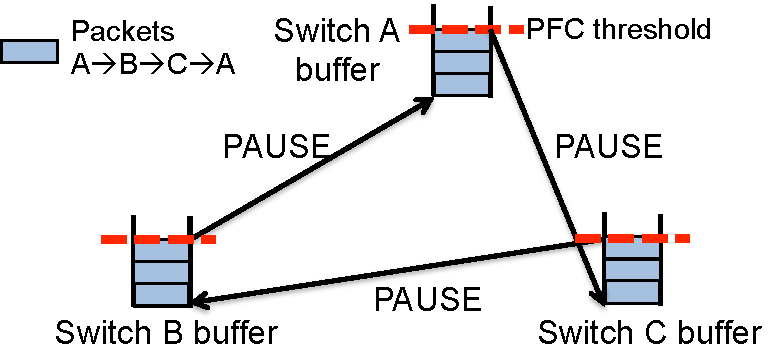
\includegraphics[width=0.45\textwidth] {figs/deadlock}
		\vspace{-1em}
		\caption{A simple (but contrived) example to illustrate CBD formation
		without routing loop.}
		\vspace{-1em}
		\label{fig:basic_deadlock}
\end{figure}

\section{Background}
\label{sec:background}

We now provide a brief primer on RDMA, RoCE, the problem of deadlocks and prior
work in this area.

{\bf RDMA and RoCE:} Remote Direct Memory Access (RDMA) technology offers high
throughput, low latency and low CPU overhead, by bypassing end-host networking
stacks. Instead, Network Interface Cards(NICS) transfer data in and out of
pre-registered memory buffers at the two end hosts.  In modern data centers,
RDMA is deployed using RDMA over Converged Ethernet V2 (RoCE)
standard~\cite{roce,rroce}

{\bf PFC:} RoCE needs a lossless L2 layer for optimal performance. This is
accomplished in Ethernet networks using the Priority Flow Control (PFC)
mechanism~\cite{pfc}.  Using PFC, a switch can pause an incoming link when its
ingress buffer occupancy reaches a preset threshold. As long as sufficient
``headroom'' is reserved to buffer packets that are in flight during the time
takes for the PAUSE to take effect, no packet will be dropped due to buffer
overflow~\cite{cisco-whitepaper,dcqcn}. 

The PFC standard defines 8 classes\footnote{Although, only one or two can be
used in practice -- see \S\ref{subsec:pfcheadroom}.}, called priorities~\footnote{The word priority is a
misnomer. There is no implicit ordering among priorities -- they are really just
separate classes.}. Packets in each priority are buffered separately, and PAUSE
messages carry this priority.  When a packet arrives at port $i$ of switch $S$
with priority $j$, it is enqueued in queue $j$ of port $i$. If the queue length
now exceeds the PFC threshold, a pause message (XOFF) is sent to the upstream
switch connected to port $i$. The message carries priority $j$. The upstream
switch then stops sending packets with priority $j$ to switch $S$ on port $i$ until a resume
message (XOFF) with priority $j$ is received.

PFC prevents buffer overflow, but it can lead to deadlocks.

%% Since PAUsing is carried out
%% on a per-ingress port, and not on a per-flow basis, problems such as unfairness
%% and head-of-the-line blocking may occur~\cite{dcqcn}. The PFC standard defines 8
%% classes (called priorities), where packets in class are buffered separately, to
%% mitigate these problems~\cite{dcqcn}. However, sine each priority needs its own
%% dedicated headroom, typically, no more than two or three priorities are
%% used~\cite{rdmaatscale}.

{\bf Deadlock:} Deadlock forms when paused links form a cycle
(Figure~\ref{fig:deadlock_example}). Once formed,
deadlock is ``permanent'' in the sense that it will continue to exist even if no
new traffic is injected into the loop. Deadlocks in PFC-based networks (or more
generally, in credit-flow networks) are a well-known problem. It is not merely a
theoretical problem -- it has been reported in practice~\cite{rdmaatscale}.

It is well known that Circular Buffer Dependency (CBD) is a {\em necessary}
condition for deadlock formation~\cite{tcp-bolt,hu2016deadlocks}. {\em
Sufficient} condition for deadlock formation in PFC networks have yet to be
fully understood~\cite{hu2016deadlocks}. 

{\bf Prior work on deadlock avoidance:} Prior work on deadlock management falls
in two categories: deadlock avoidance, or deadlock detection and resolution. Our
focus in this paper is on deadlock avoidance.  Since {\em sufficient} conditions
for deadlock formation are not well characterized, deadlock avoidance schemes
focus on preventing CBD for occurring. This is done either by limiting or
modifying routing~\cite{tcpbolt} to avoid CBD, or by careful buffer
management~\cite{xxx}. 

However, these schemes fail to meet one or more of the three key challenges:
$(i)$ they cannot be deployed with existing routing, or, $(ii)$ they do not deal
with dynamic nature of data center networks, or, $(iii)$ they require excessive
switch buffers or number of priorities. 

We now describe these three challenges in more detail. See \S\ref{sec:related}
for a detailed review of prior work.

%% Prior work on deadlock formation fails to meet the three challanges: first, they
%% do not work with To avoid such deadlocks, {\em deadlock-free
%% routing}~\cite{tcpbolt} has been proposed. It guarantees that (if the routing
%% configuration is correct,) any traffic does not cause deadlock.
%% 
%% Unfortunately, achieving deadlock-free routing is inefficient, and may not even
%% be viable. Deadlock-free routing is achieved by eliminating Cyclic Buffer
%% Dependency (CBD)~\cite{deadlockfree}.  However, ensuring that there is never any
%% CBD is challenging.
%% 
%% First, deadlock-free routing largely limits the choice of topology. For example,
%% Stephens et al. \cite{tcpbolt} proposes to only use tree-based topology and
%% routing, and shows that it is deadlock-free.  However, there are a number of
%% other datacenter topologies and routing schemes that are not
%% tree-based~\cite{bcube, camcube, jellyfish}, and do not have deadlock-free
%% guarantee.
%% 
%% Second, due to bugs or misconfiguration, deadlock-free routing configuration may
%% turn into deadlock-vulnerable. In fact, recent work has observed a PFC deadlock
%% case in real-world tree-based datacenter\cite{rdmascale}, caused by the
%% (unexpected) flooding of lossless class traffic.  Furthermore, there are
%% multiple reports of routing loops due to misconfiguration in today's production
%% datacenters~\cite{everflow, libra}. If lossless traffic encounters any of these
%% loops, CBD is unavoidable.  
%% 
%% Indeed, a recent paper~\cite{hu2016deadlocks} argued that preventing CBD is
%% quite difficult, so instead we should focus on defining and preventing
%% ``simpler''{\em sufficient} conditions to avoid deadlock. 
%% 
%% In this paper, we show that it is indeed possible to prevent CBD, in any
%% topology, without any changes to the underlying routing protocol, using existing
%% data center hardware. 





\section{Deadlock case study}\label{sec:casestudy}

In this part, we present our simulation study about three deadlock cases, and demonstrate that 1) cyclic buffer dependency is not a sufficient and necessary condition for deadlock; 2) simultaneous cyclic pause is not sufficient to create a permanent deadlock.

\begin{figure*}[t]
%\vspace{-0.1in}
\centering

\subfloat[short for lof][Topology and flows.] {
    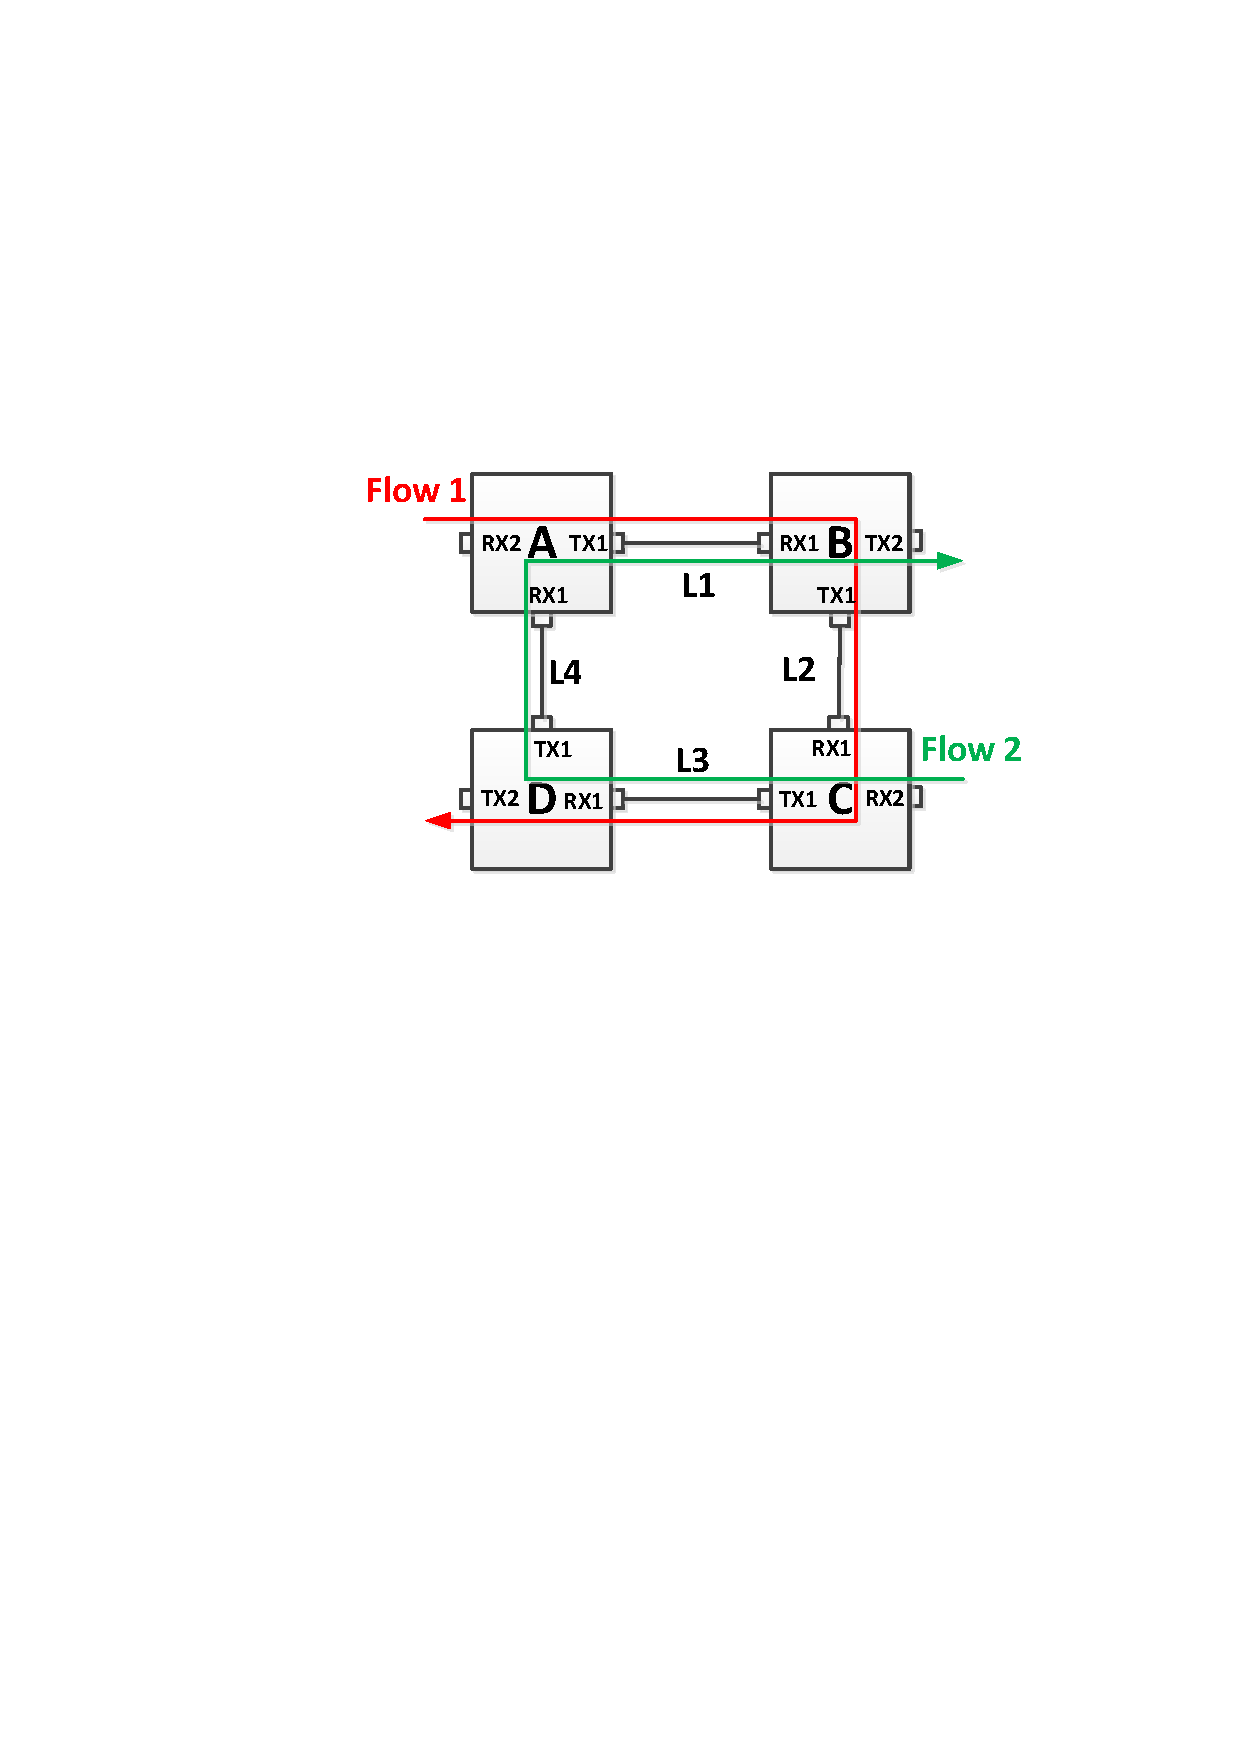
\includegraphics[width=0.35\textwidth] {figs/case1_topo.pdf}
}
\subfloat[short for lof][Buffer dependency graph.]{
    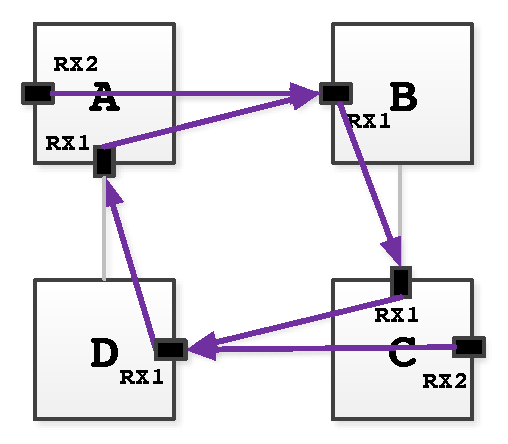
\includegraphics[width=0.24\textwidth] {figs/case1_buffer_dependency.pdf}
}
\subfloat[short for lof][Pause events at four links.]{
    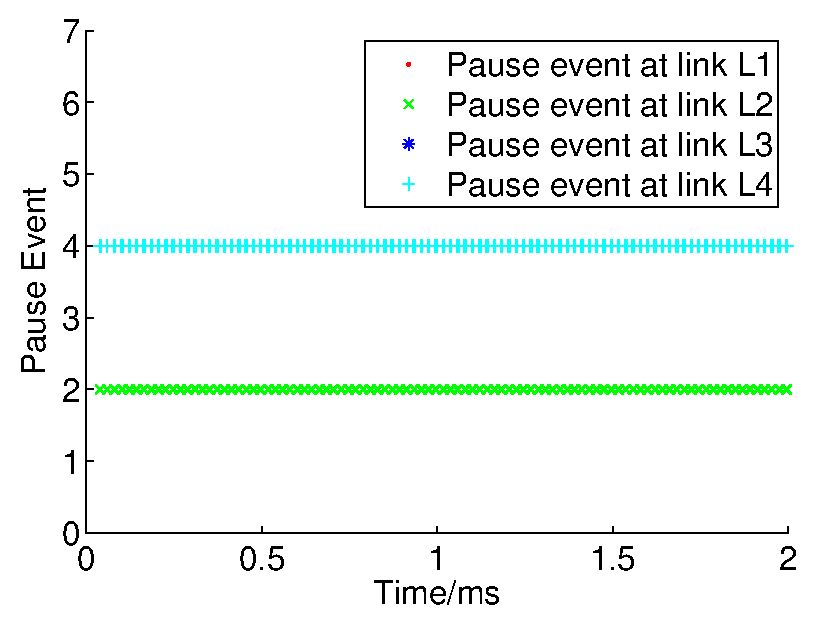
\includegraphics[width=0.3\textwidth] {figs/case1_pause.eps}
}

\subfloat[short for lof][Buffer occupancy at switch A.] {
    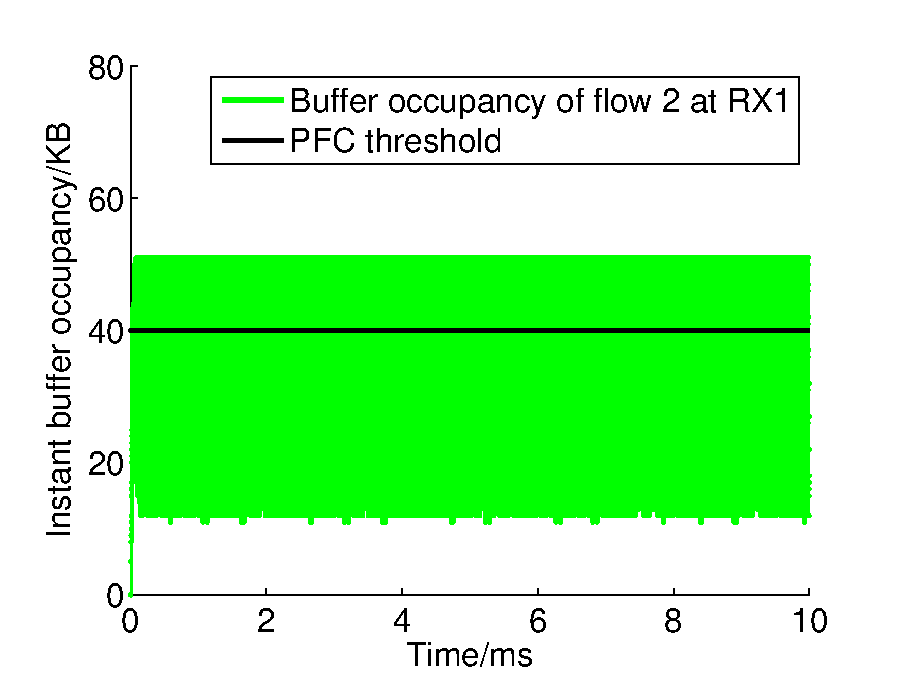
\includegraphics[width=0.25\textwidth] {figs/case1_buffer_occupancy_A.eps}
}
\subfloat[short for lof][Buffer occupancy at switch B.] {
    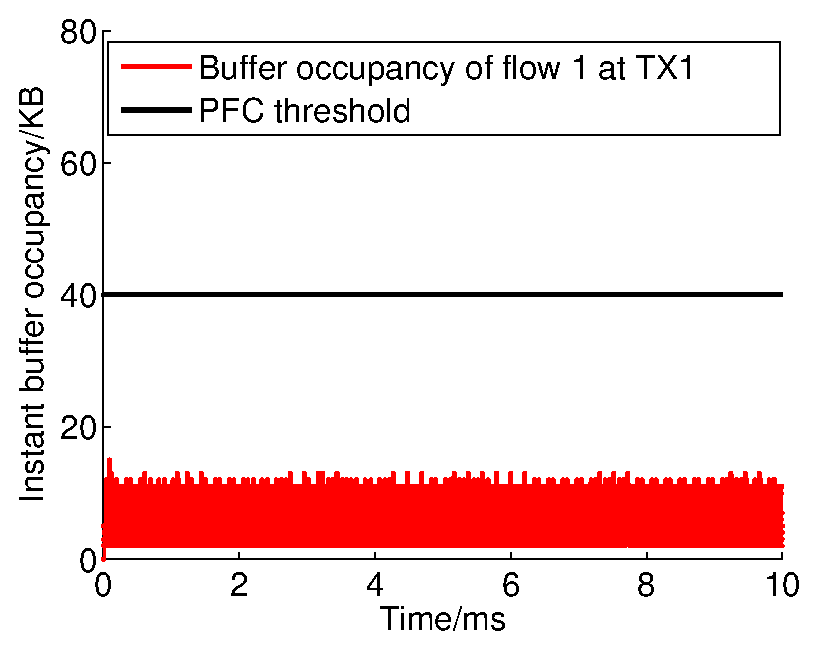
\includegraphics[width=0.25\textwidth] {figs/case1_buffer_occupancy_B.eps}
}
\subfloat[short for lof][Buffer occupancy at switch C.] {
    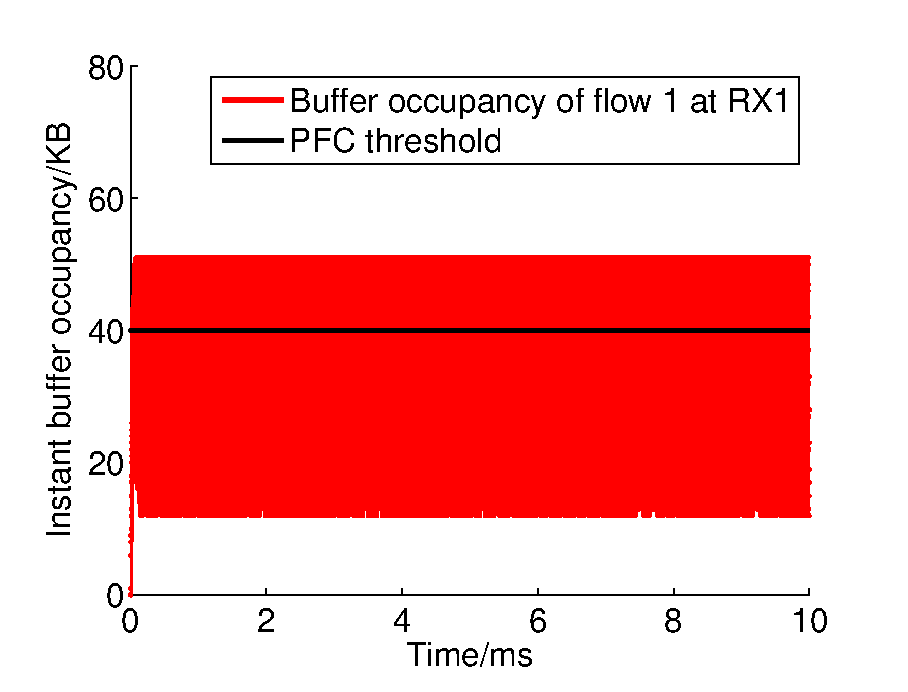
\includegraphics[width=0.25\textwidth] {figs/case1_buffer_occupancy_C.eps}
}
\subfloat[short for lof][Buffer occupancy at switch D.] {
    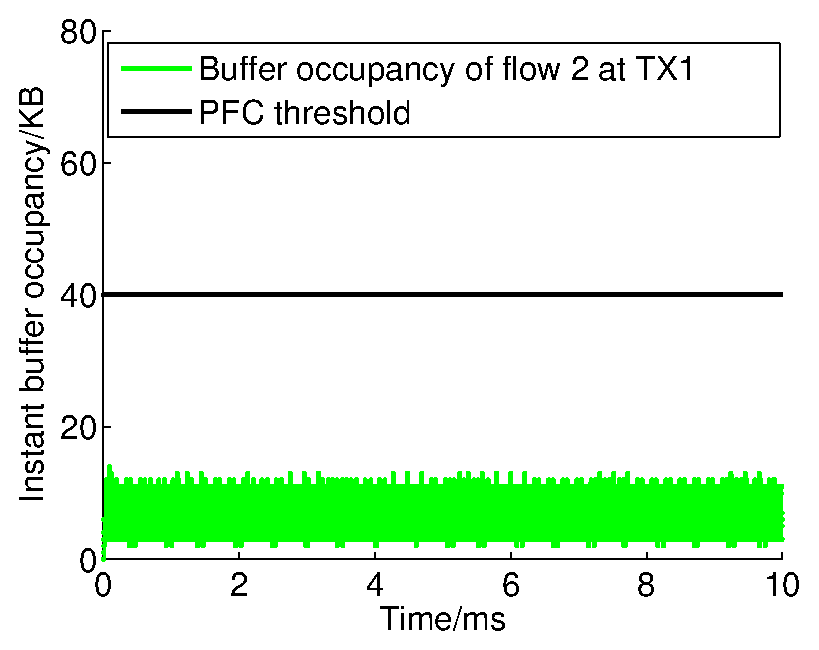
\includegraphics[width=0.25\textwidth] {figs/case1_buffer_occupancy_D.eps}
}

\caption{Deadlock case 1.}\label{fig:case1}

\end{figure*}

 \textbf{Simulation setup}: To create a well controlled experimental environment for deadlock analysis, we did our deadlock case study using packet-level NS-3 simulations. 
 
 In our modified NS-3 simulator, we implement PFC protocol (i.e., IEEE 802.1 Qbb protocol). Note that most modern commodity switches are output-queued, while PFC works in a per ingress queue fashion. Basically, for each ingress queue, the switch will maintain a counter to track its instant virtual queue length (i.e., bytes of buffered packets received by this ingress queue). Once the queue length of an ingress queue exceeds the pre-configured PFC threshold, a pause frame will be sent to the corresponding upstream device. The upstream device then stop sending any packet to this ingress queue unless 1) the pause frame has expired; 2) or it has received a resume frame from this ingress queue.
 
 In our simulations, link capacity of all links is 40Gbps. All the switches have 12MB buffer. PFC threshold is statically set to 40KB for each ingress queue.


\begin{figure*}[t]
%\vspace{-0.1in}
\centering

\subfloat[short for lof][Topology and flows.] {
    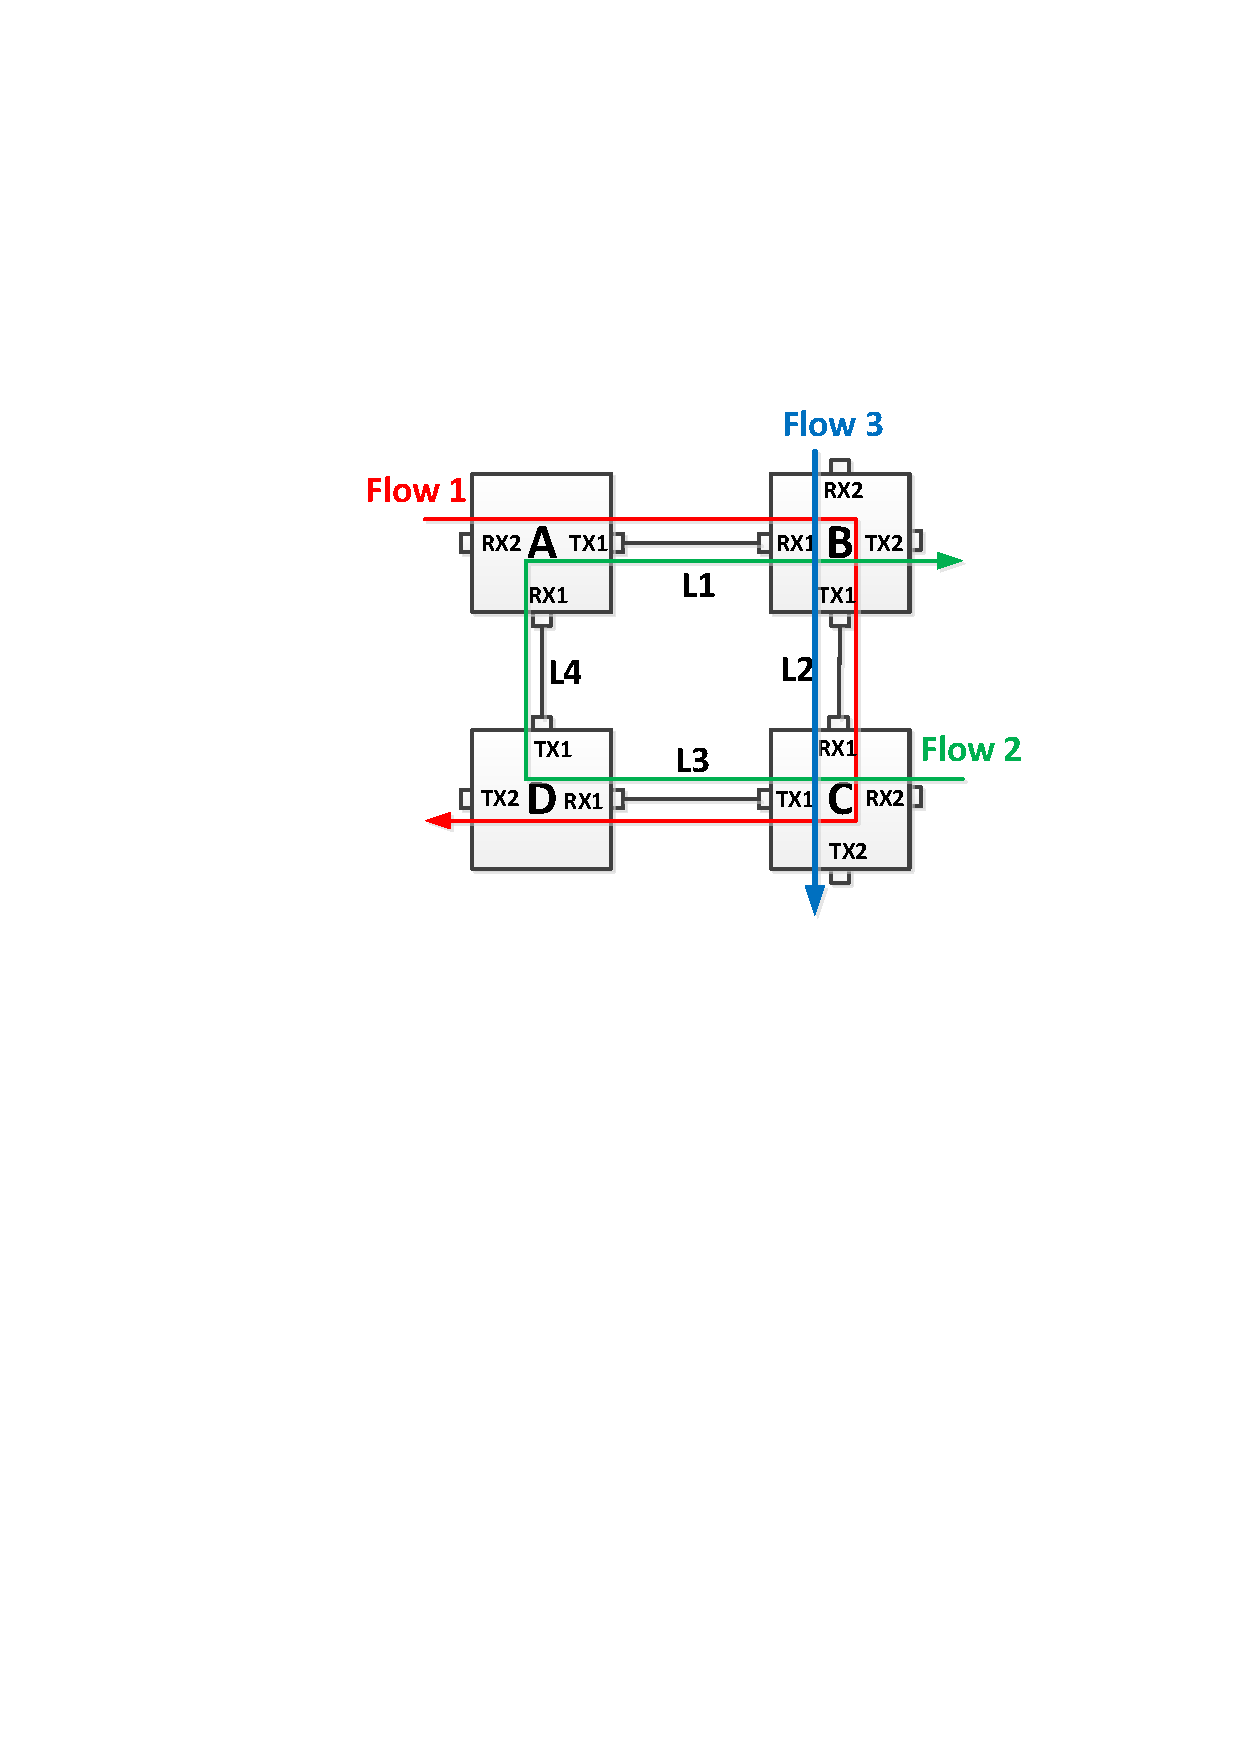
\includegraphics[width=0.37\textwidth] {figs/case2_topo}
}
\subfloat[short for lof][Buffer dependency graph.]{
    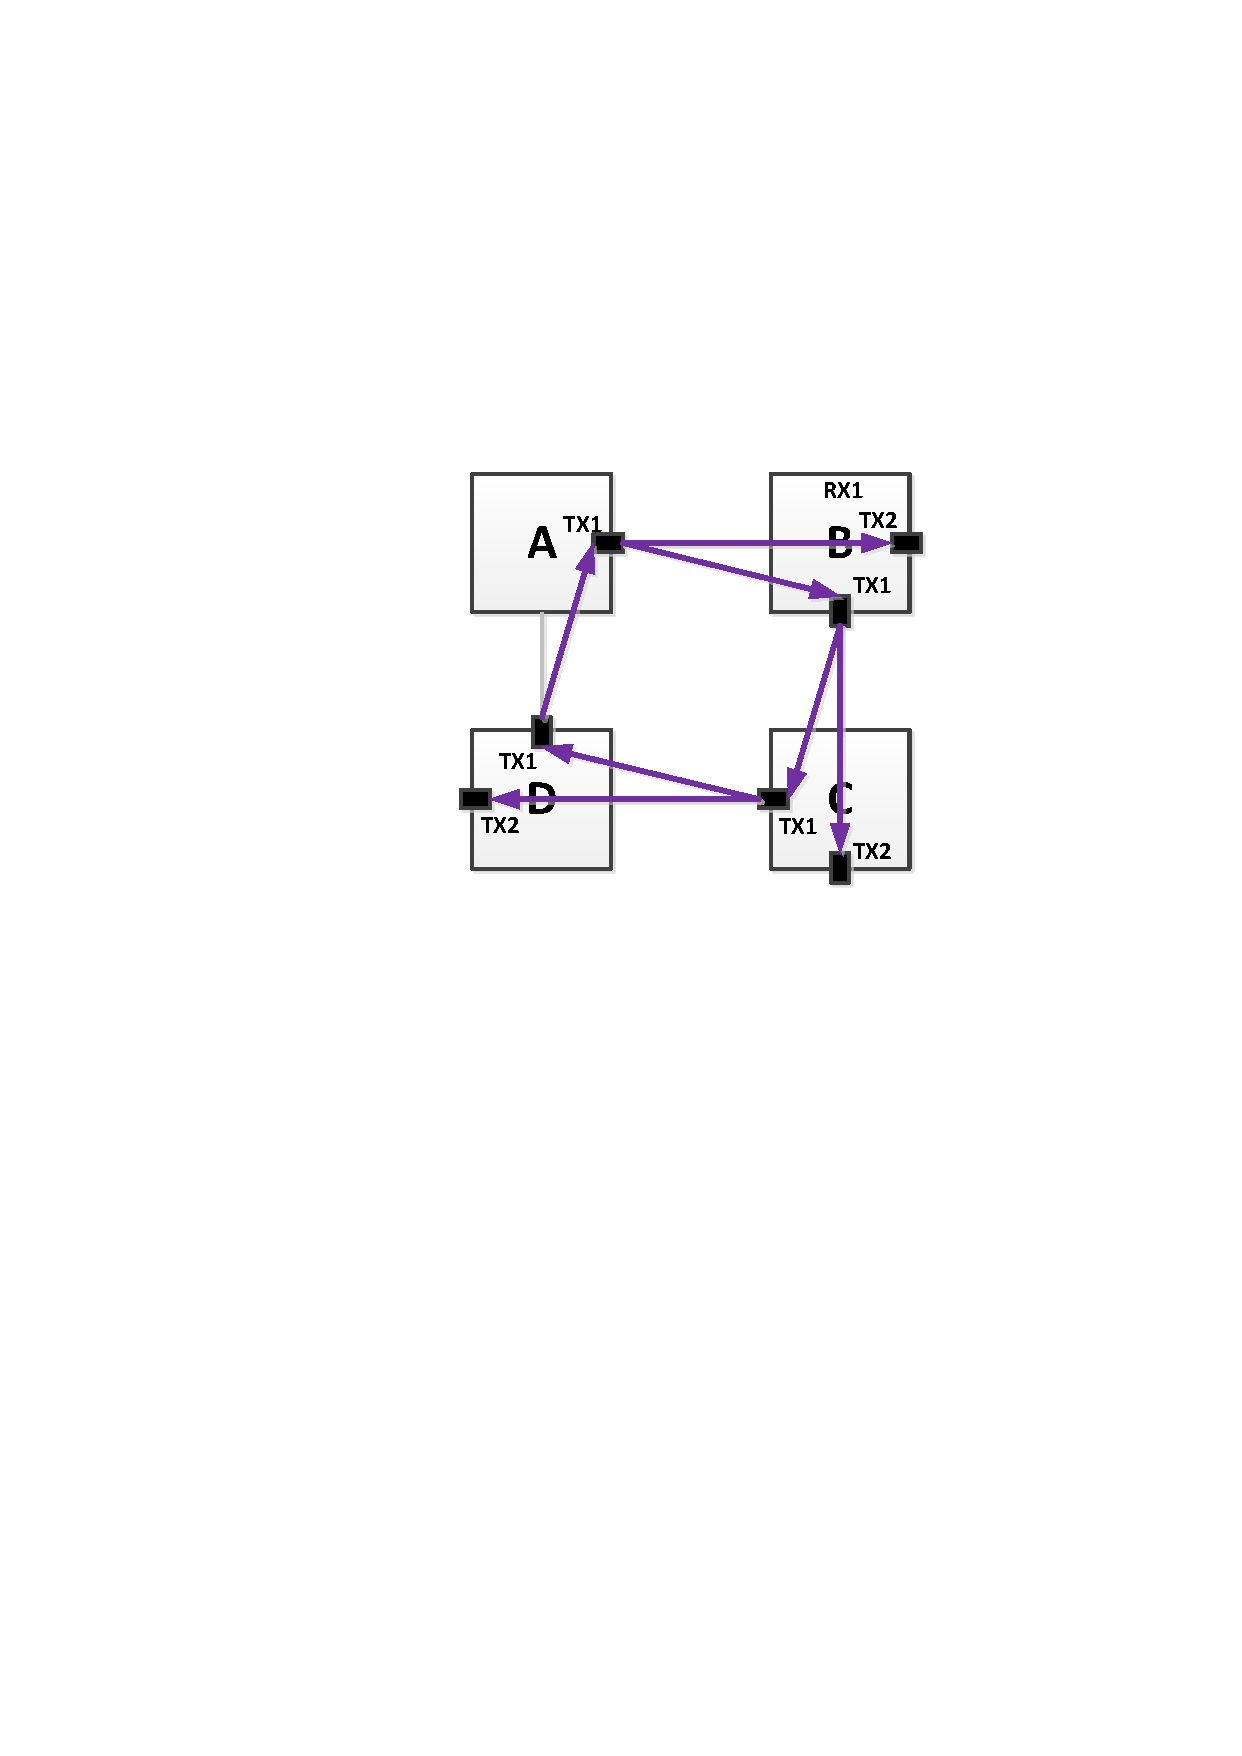
\includegraphics[width=0.27\textwidth] {figs/case2_buffer_dependency}
}
\subfloat[short for lof][Pause events at four links.]{
    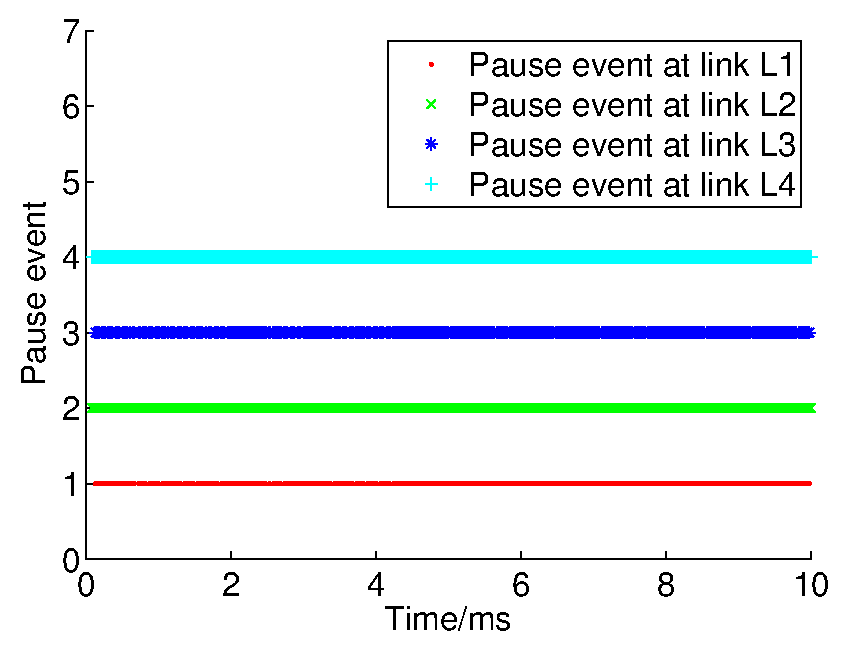
\includegraphics[width=0.3\textwidth] {figs/case2_pause.eps}
}


\caption{Deadlock case 2.}\label{fig:case2}

\end{figure*}

\textbf{Case 1:} In this case, as shown in Fig.~\ref{fig:case1}(a), we let two flows run over four switches A, B, C and D. Flow 1 starts at a host (not shown) attached to A, passes through B and C, and ends at a host attached to D. Flow 2 starts at a host attached to C, passes through D and A, and ends at a host attached to B. In the figure, RX represents input queue (or port), while TX represents output queue (or port). To evaluate whether there will be deadlock in the worst case, both flows are UDP flows with infinite traffic demand.

Buffer dependency graph of case 1 is drawn in Fig.~\ref{fig:case1}(b). Each directed line represents a buffer dependency from the source TX to the destination TX. For example, packets buffered in TX1 of A will be sent to either TX1 or TX2 of B, so in Fig.~\ref{fig:case1}(b), two directed lines are drawn there between A and B. Similarly, we can draw the dependency lines between other switches. As we can see in Fig.~\ref{fig:case1}(b), there is a cyclic buffer dependency among the four switches, i.e., dependencies from TX1 of A to TX1 of B, then to TX1 of C, then to TX1 of D, and finally back to TX1 of A.

In Fig.~\ref{fig:case1}(c), we plot the PFC pause events at four links L1, L2, L3 and L4. Basically, if link Li (i=1,2,3,4) is paused at time t, we plot a point at location (t, i). Pause events at different links are plotted with different colors and of different heights. As we can observe, links L2 and L4 are paused continuously, while the other two links L1 and L3 never get paused. In this case, deadlock will never occur as no packet will be paused permanently.

To understand the pause pattern in Fig.~\ref{fig:case1}(c), we sample the instant buffer occupancy of both flows at TX1 queues of A, B, C and D every 1us. In Fig.~\ref{fig:case1}(d), we draw the instant buffer occupancy of flow 2 at TX1 of A. Buffer occupancy of flow 1 is not drawn in Fig.~\ref{fig:case1}(d) as it does not contribute to the pause of link L1 (Note that PFC works in a per ingress queue fashion). 

Similarly, in Fig.~\ref{fig:case1}(e), Fig.~\ref{fig:case1}(f) and Fig.~\ref{fig:case1}(g), we draw the instant buffer occupancy of interested flows at TX1 queues of B, C and D, respectively. As flow 1 and flow 2 are symmetric, we only present the analysis for Fig.~\ref{fig:case1}(d) and Fig.~\ref{fig:case1}(e) to show why Link L4 is paused continuously but link L1 never gets paused.

As shown in Fig.~\ref{fig:case1}(d), buffer occupancy of flow 2 at TX1 of A fluctuates between 10KB and 55KB around the PFC threshold, so link L4 will get paused intermittently. In contrast, buffer occupancy of flow 1 at TX1 of B is well below the PFC threshold (fluctuates between 0KB and 18KB), hence link L1 will never be paused.

%In Fig.~\ref{fig:case1}(a), packets of flow 1 and flow 2 will build up at TX1 of A as both flows are competing for the capacity of link L1. Once the buffer occupancy of flow 2 exceeds the PFC threshold, RX1 of A will generate a pause frame to TX1 of D to stop packet transmission over link L4.
%
%After link L4 is paused, buffer occupancy of flow 2 will decrease as no more packets can be received by RX1 of A. Once the buffer occupancy of flow 2 is below the PFC threshold at switch A, link L4 will be resumed. Then buffer occupancy of flow 2 will start to increase again. This is why in
%
%Since packets of flow 1 buffered in TX1 of B can get transmitted at full link speed when link L2 is not paused, TX1 queue of B can not easily build up. As we can see in Fig.~\ref{fig:case1}(e), buffer occupancy of flow 1 at TX1 of B fluctuates between 0KB and 18KB, which . Hence as we can see in Fig.~\ref{fig:case1}(c), link L1 is never paused by RX1 of C.


\textbf{Observation 1:} Deadlock may not occur when cyclic buffer dependency exists in the network. Cyclic buffer dependency is just a necessary condition for deadlock.



\textbf{Case 2:} as shown in Fig.~\ref{fig:case2}(a), in the second case, in addition to case 1, we add another flow (flow 3) to run over switches B and C in sequence. All the three flows are UDP flows with infinite traffic demand. Buffer dependency graph of case 2 is drawn in Fig.~\ref{fig:case2}(b). Compared with case 1, one additional dependency from TX1 of B to TX1 of C is added.

Pause events at four links L1, L2, L3 and L4 are plotted In Fig.~\ref{fig:case2}(c). As we can see, in this case four links are all paused. To check whether deadlock will occur in this case, we stop the three flows after a sufficient long period (1000ms). What we find is that, pause events are continuously generated at all the four links even after three flows stop sending new packets (not shown in the figure). This means that a deadlock has been created among switches A, B, C and D.

In the next, we will explain why deadlock can be created by adding one additional flow to the network. After adding flow 3, packets of flow 1 buffered in TX1 of B can no longer get transmitted at full link speed due to the contention with packets of flow 3. Packets of flow 1 will then build up at TX1 of B. Once the packets of flow 1 buffered at TX1 of B exceed the PFC threshold, RX1 of B will send a pause frame to TX1 of A to pause Link L1. The pause on link L1 will help packets to build up at TX1 of A, and has a cascade effect on link L4. Due to the pause at link L1, link L4 will get paused more frequently. Then packets of flow 2 are easier to build up at TX1 of D. Once the PFC threshold is triggered at D, link L3 also get paused. So in case 2, pause events can occur at all the four links.

Once all the four links are paused simultaneously, there is a chance that no link can get resumed. For example, it is possible that when simultaneous pause happens, at switch A and switch B, the first packet buffered in the head of TX1 is a packet of flow 1, and meanwhile, at switch C and switch D, the first packet buffered in the head of TX1 is a packet of flow 2. If the above condition occurs, no link can get resumed as all the TX1 queues are waiting for its downstream neighbors to release some buffer to break the standstill condition.

\textbf{Observation 2:} Deadlock will occur when all the links in a cycle are paused simultaneously and no link can get resumed.


\begin{figure*}[t]
%\vspace{-0.1in}
\centering

\subfloat[short for lof][Topology and flows.] {
    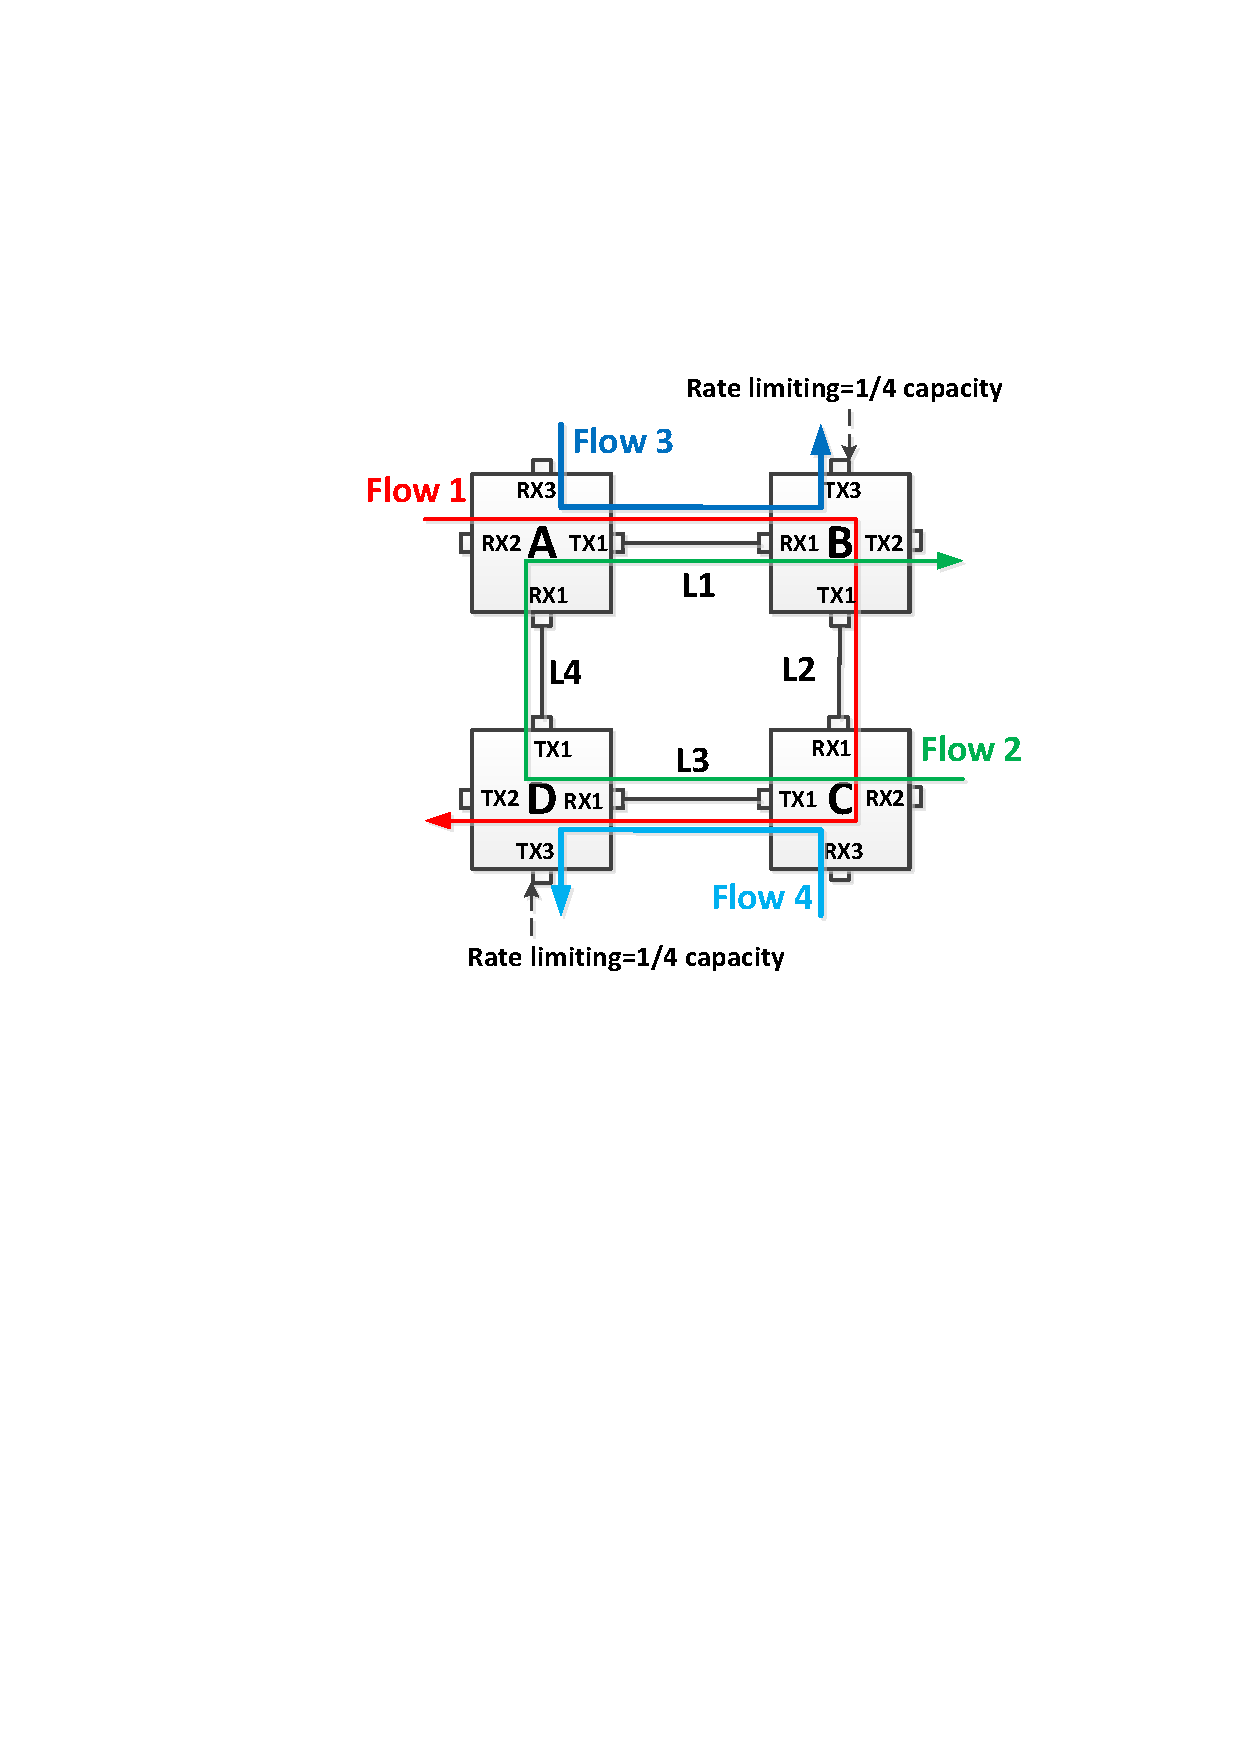
\includegraphics[width=0.37\textwidth] {figs/case3_topo}
}
\subfloat[short for lof][Buffer dependency.]{
    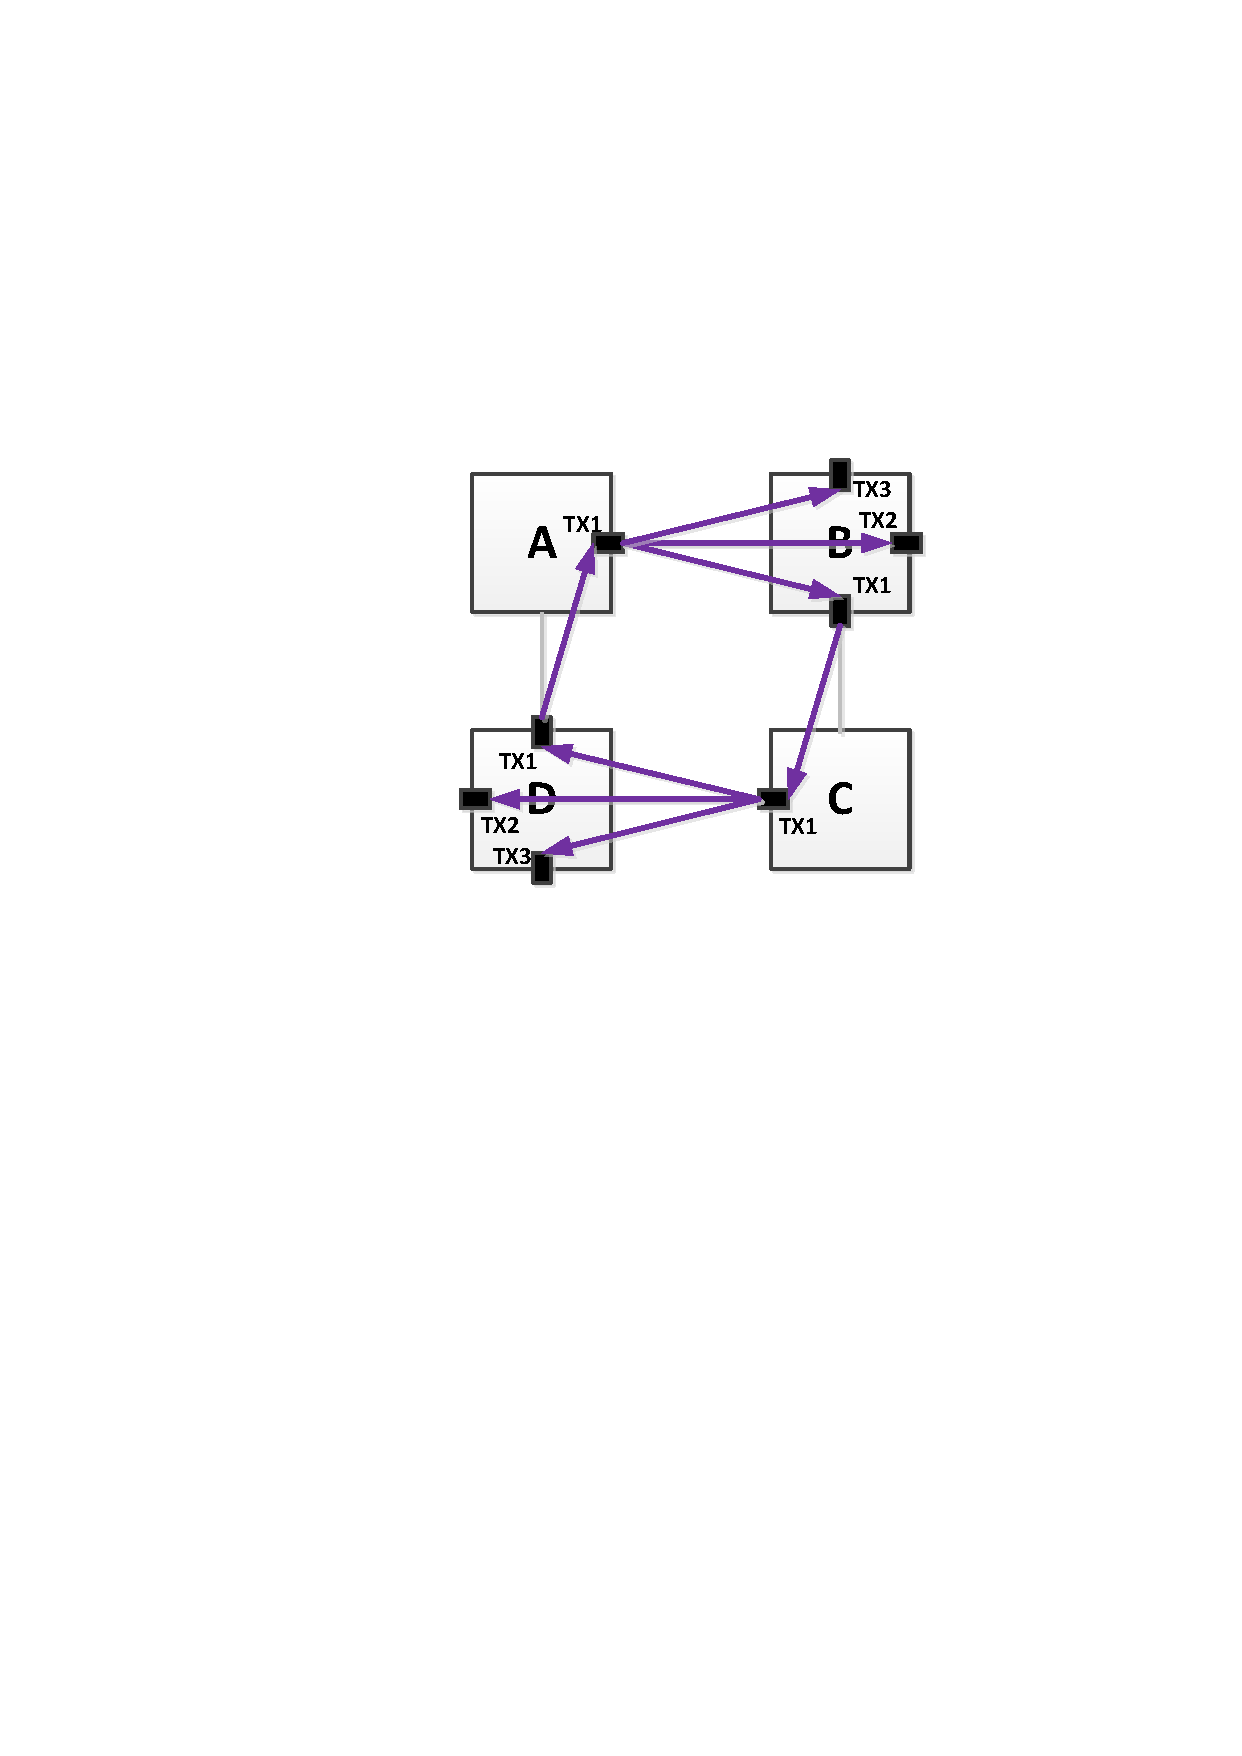
\includegraphics[width=0.28\textwidth] {figs/case3_buffer_dependency}
}
\subfloat[short for lof][Pause events at four links.]{
    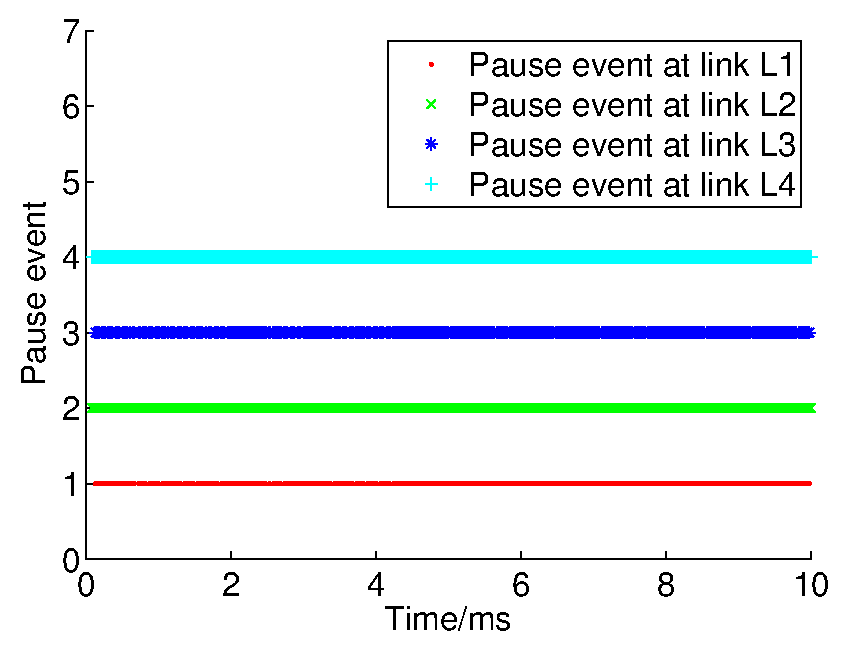
\includegraphics[width=0.3\textwidth] {figs/case3_pause.eps}
}

\subfloat[short for lof][Buffer occupancy of flow 2 at switch A.] {
    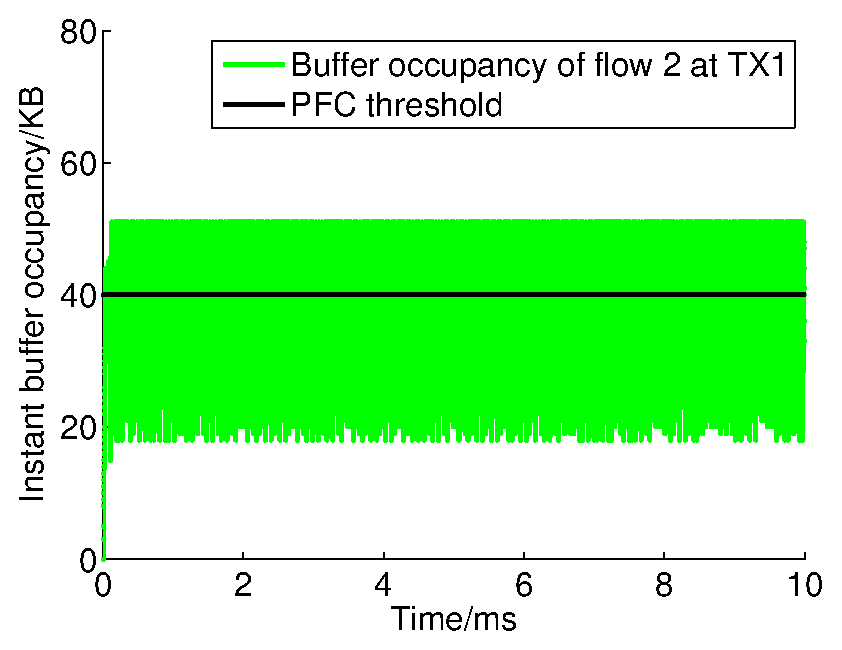
\includegraphics[width=0.33\textwidth] {figs/case3_buffer_occupancy_A.eps}
}
\subfloat[short for lof][Buffer occupancy of flow 1 at switch B.] {
    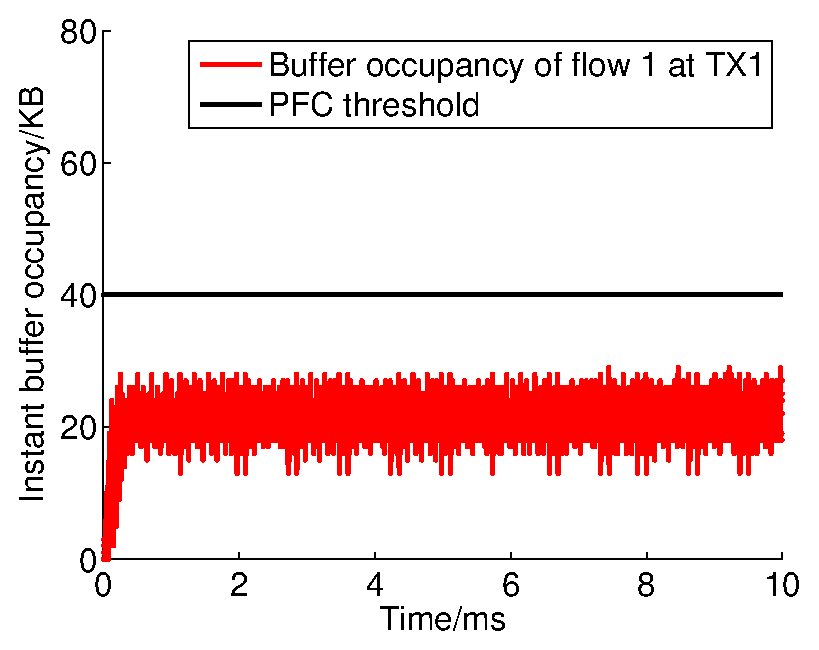
\includegraphics[width=0.33\textwidth] {figs/case3_buffer_occupancy_B1.eps}
}
\subfloat[short for lof][Buffer occupancy of flow 3 at switch B.] {
    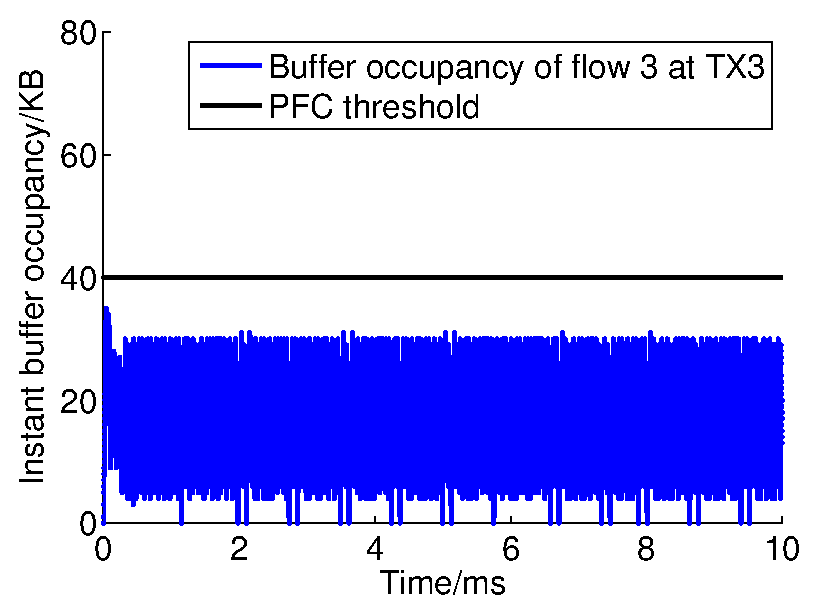
\includegraphics[width=0.33\textwidth] {figs/case3_buffer_occupancy_B3.eps}
}

\caption{Deadlock case 3.}\label{fig:case3}

\end{figure*}

\textbf{Case 3:} In this case, we will show that even if all the four links are paused simultaneously, it is not guaranteed that a deadlock will be created. As shown in Fig.~\ref{fig:case3}(a), in addition to case 1, we add another two flows (flow 3 and flow 4). Flow 3 starts at a host attached to A, passes through A and B, and ends at a host attached to B. Flow 4 is a symmetric flow of flow 3 that runs over C and D. All the four flows are UDP flows with infinite traffic demand. Two rate limiters are added at TX3 queues of B and D to ensure that rates of flow 3 and flow 4 will not exceed $1/4$ of the link capacity. Buffer dependency graph of case 3 is drawn in Fig.~\ref{fig:case3}(b). Compared with case 1, two additional buffer dependencies from TX1 queues to TX3 queues are added.

Pause events at four links L1, L2, L3 and L4 are plotted In Fig.~\ref{fig:case3}(c).  As we can see from the figure, all the four links are paused continuously. However, we find that once we stop the flows, all the links get resumed and buffer occupancy of four switches soon becomes zero. This indicates that deadlock cannot be created in case 3.

To find out why there is no deadlock in case 3, we draw the instant buffer occupancy of 3 flows at switches A and B in Fig.~\ref{fig:case3}(d), Fig.~\ref{fig:case3}(e) and Fig.~\ref{fig:case3}(f). Here we omit the buffer occupancy condition of switches C and D as the topology and the flows are symmetric.

As shown in Fig.~\ref{fig:case3}(d), at TX1 of A, the buffer occupancy of flow 2 exceeds the PFC threshold, so link L4 will get paused. To understand why link L1 is also paused, we need to consider the buffer occupancy of flow 1 and flow 3 at switch B. The reason is that packets received by RX1 of B are possible to be queued at both TX1 and TX3 (note that there is a rate limiter on TX3). As long as the sum of the buffer occupancies of both TX queues exceeds the PFC threshold, link L1 will get paused. As we can see in Fig.~\ref{fig:case3}(e) and Fig.~\ref{fig:case3}(f), although individually buffer occupancy of either TX1 or TX3 is less than the PFC threshold, their sum is larger than the PFC threshold. Hence link L1 is paused.

As both TX1 and TX3 contribute to the pause on link L1, to create a deadlock, we need to ensure that packets buffered at both TX queues cannot get resumed. However, packets buffered at TX3 can always get transmitted within a finite time as it is not involved in any cyclic buffer dependency. This explains why when we stop the flows, all the four links can be resumed from the pauses. 


\textbf{Observation 3:} even if all the links in a cycle are paused simultaneously, it is not sufficient to create a permanent deadlock.

%\subsection{Deadlock problem in RDMA DCNs}\label{subsec:deadlock_problem}
%
%Once a loop occurs in a network, packets of some flows will be caught in the loop and traverse the same links multiple times until they are dropped due to Time-to-Live (TTL) expiration. Apart from causing packet drops, loops will also waste some link bandwidth as well as increase the end-to-end delay for the flows traversing some link(s) in the loop (but not caught by the loop).
%
%\begin{figure}[t]
%\centering
%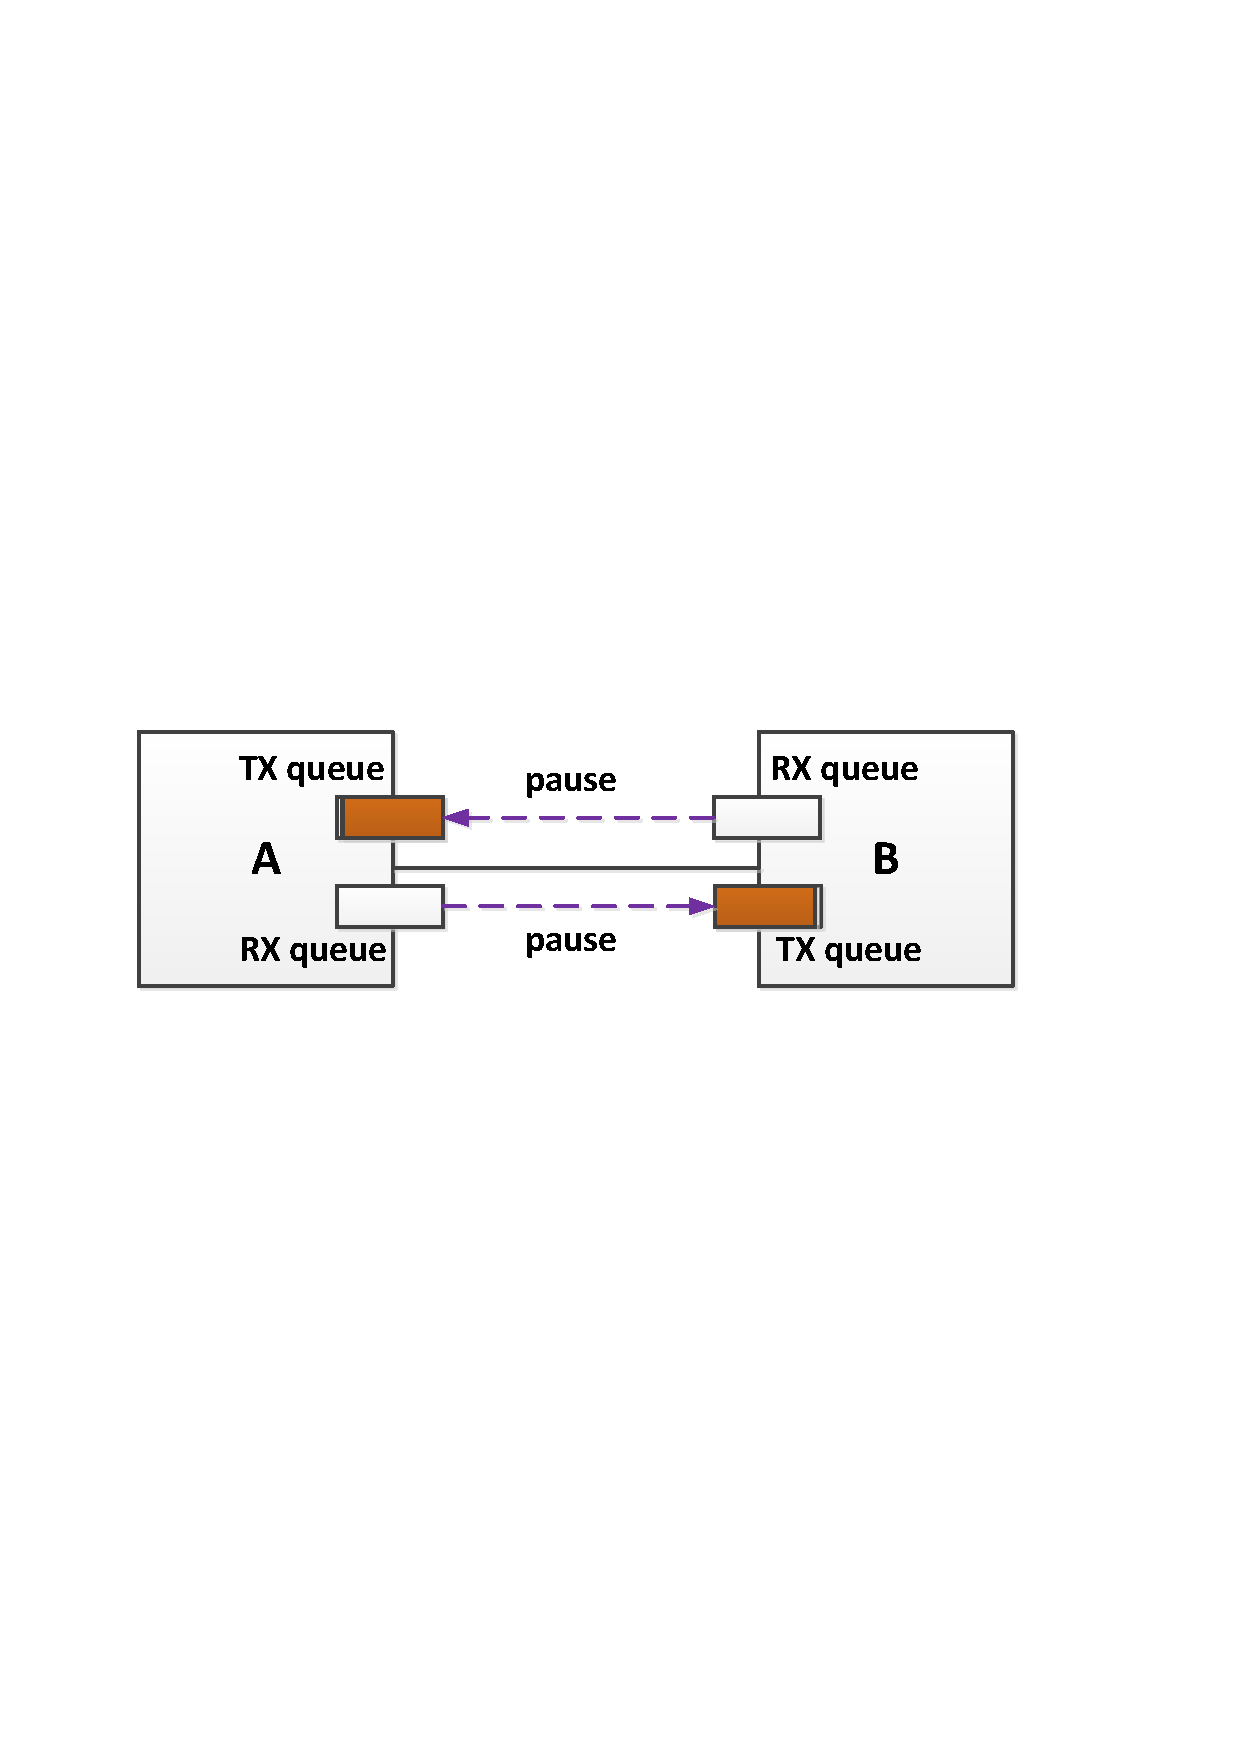
\includegraphics[width=0.45\textwidth,center]{figs/deadlock_example.pdf}
%\caption[Optional caption for list of figures]{An example of loop induced deadlock: there is a loop between switch A and switch B. Both TX queues (egress queues) are paused by PFC as no buffer are available at both switches to accommodate more packets.}
%\label{fig:loop_deadlock}
%\end{figure}
%
%In a lossy network, the impact of a loop is not fatal and can be completely eliminated as long as the loop is removed from the network. In contrast, in a lossless network, if packets enter a loop faster than they get dropped in the loop due to TTL expiration, packets will occupy the buffer of all the switches in the loop, and then a deadlock is created. When a deadlock occurs, each switch in the loop is paused by its downstream switch, and at the same time pauses its upstream switch due to the lack of available buffer to accept more packets. Once such a circular buffer dependency is created, the deadlock condition will hold persistently even after the loop is eliminated.
%
% Under deadlock condition, no packets can move along the links in the loop, and more and more devices outside the loop will be paused due to the cascade effect of PFC. If a deadlock is created in the core of the network, it is very likely to bring the whole data center into a deadlock state.
%
%A simple deadlock example is shown in Fig.~\ref{fig:loop_deadlock}. In this example, there is a routing loop between switch A and switch B. Packets enter this loop at a sufficient large rate and soon occupy all the available buffer of both switches. Then Both TX queues (egress queues) will be paused by PFC PAUSE frames and a deadlock is created. As we can see, this deadlock cannot be resolved by eliminating the routing loop as packets are already queued in the TX queues and can never reach the next-hop switch to escape from the loop.
%
%\subsection{Sufficient condition for deadlock creation}\label{subsec:deadlock_condition}
%
%In this part, we analyze the sufficient condition to create a deadlock when there is a loop in the network.
%
%At first, we consider the maximum packet drain rate in a loop regarding TTL expiration. Let $n$ the number of switches in a loop, $B$ be the link bandwidth and $k_{TTL}$ be the TTL value of packets before they enter the loop. Each time a packet traverses one switch, its TTL value will be reduced by 1.
%
%The maximum packet drain rate is achieved when no switch is paused by PFC PAUSE frame and each switch is sending packets to its next-hop in the loop at the rate of $B$. So the maximum packet drain rate $r^{max}_d$ is equal to $nB/k_{TTL}$. here $nB$ can be viewed as the maximum packet ``flowing" rate in the loop, while $1/k_{TTL}$ captures the information that a packet will be dropped after it has traversed $k_{TTL}$ hops of switches in the loop.
%
%Let $r_{in}$ be the injection rate of packets into the loop. One sufficient condition to create a deadlock in a lossless network is that: there is a loop
%in the network, and condition $r_{in} > r^{max}_d$ holds for a sufficient long period until a circular buffer dependency is created in the loop.
%
%\begin{figure}[t]
%\centering
%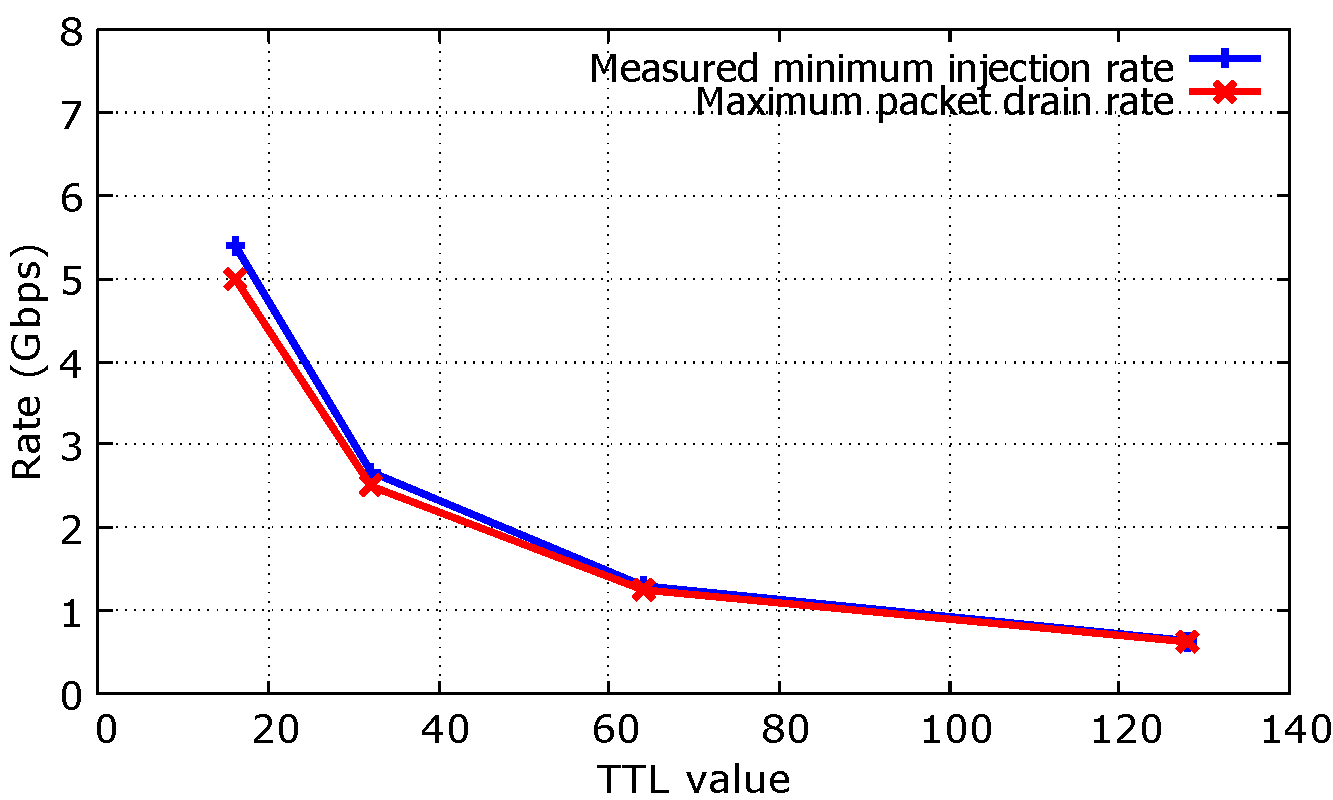
\includegraphics[width=0.5\textwidth,center]{figs/r_and_rdrain.pdf}
%\caption[Optional caption for list of figures]{Measurement of the minimum injection rate to create a deadlock. Both switches in the loop are Arista 7050QX32.}
%\label{fig:mrate_measurement}
%\end{figure}
%
%To verify our analysis above, we manually configure a loop between two 40Gbps switches, and measure the minimum packet injection rate that can create a deadlock. The result is shown in Fig.~\ref{fig:mrate_measurement}. As we can see, the measured minimum packet injection rate is just slightly larger than the maximum packet drain rate which is computed according to $nB/k_{TTL}$. This observation holds when TTL is set to different values.
%
%Another observation from the figure is that, setting smaller TTL can help to prevent deadlock but its benefit is limited. As shown in the figure, when TTL is set to 16 which is already a very small value, the minimum injection rate is only about 6Gbps.
%
%\subsection{Analysis of the time to create a deadlock}\label{subsec:deadlock_condition}
%
%In this part, we analyze and measure the time to create a deadlock when the sufficient condition for deadlock creation is already met. Deadlock creation time is related to three factors: \textbf{packet injection rate $r_{in}$}, \textbf{packet drain rate $r_{d}$} and \textbf{PFC threshold $t_{PFC}$}.
%
%$t_{PFC}$ determines the minimum bytes of packets needed to be ``trapped" in the loop to create a deadlock, while $r_{in} - r_{d}$ can be viewed as the packet increase rate.
%
%%Packet injection rate is determined by the instant traffic demand of applications running in the data center. A larger injection rate requires less time to create a deadlock.
%%
%%As discussed above, the maximum packet drain rate will be a fixed value once $n$, $B$ and $k_{TTL}$ is determined. We find that packet drain rate will decrease significantly after packets are queued in the loop because it will take a packet much longer time to get dropped in the loop when there is queuing delay.
%
%Most modern commodity switches use a dynamic $\alpha$ algorithm to determine the value of PFC threshold: Let $\alpha$ be a parameter with the range from 0 to 1, $m$ be the total switch buffer size and $m^\prime$ be the amount of buffer currently occupied. For a given $\alpha$, the value of $t_{PFC}$ is dynamically computed according to the following equation $ t_{PFC} = \alpha(m - m^\prime)$. During runtime, once the queue length of an ingress queue exceeds the instant $t_{PFC}$, a PAUSE frame will be sent to its upstream device. Note that a PAUSE frame will take some time to arrive an upstream device and take effect. To avoid packet loss due to this delay, some buffer headroom must be reserved for each ingress queue, and hence the value of $m$ in the equation is usually slightly smaller than the total switch buffer size.
%
%%
%
%
% %Most modern commodity switches share memory buffer among all ports. In order to better utilize the available shared buffer in a timely fashion, instead of setting a fixed PFC threshold,
%%A PAUSE frame will take some time to arrive an upstream device and take effect. To avoid packet loss due to this propagation delay, we must reserve enough
%%buffer headroom for each ingress queue to accommodate packets a switch may receive before a PAUSE frame finally takes effect. Let $\Delta m$ be the total amount of reserved buffer headroom. The $m$ in the above equation should be modified to be $m - \Delta m$.
%%Switches and NICs will track the value of $m^\prime$ and update the value of $t_{PFC}$ during runtime.
%
%%A smaller $\alpha$ value can lead to a shorter creation time of deadlock.  This is because a smaller $\alpha$ value means a smaller PFC threshold, while a smaller PFC threshold requires less packets to trigger a switch queue to send PAUSE frames to stop its upstream neighbors.
%
%In the next, we measure the time to create a deadlock when setting different $\alpha$ and TTL values.
%
%
%\begin{figure}[t]
%\centering
%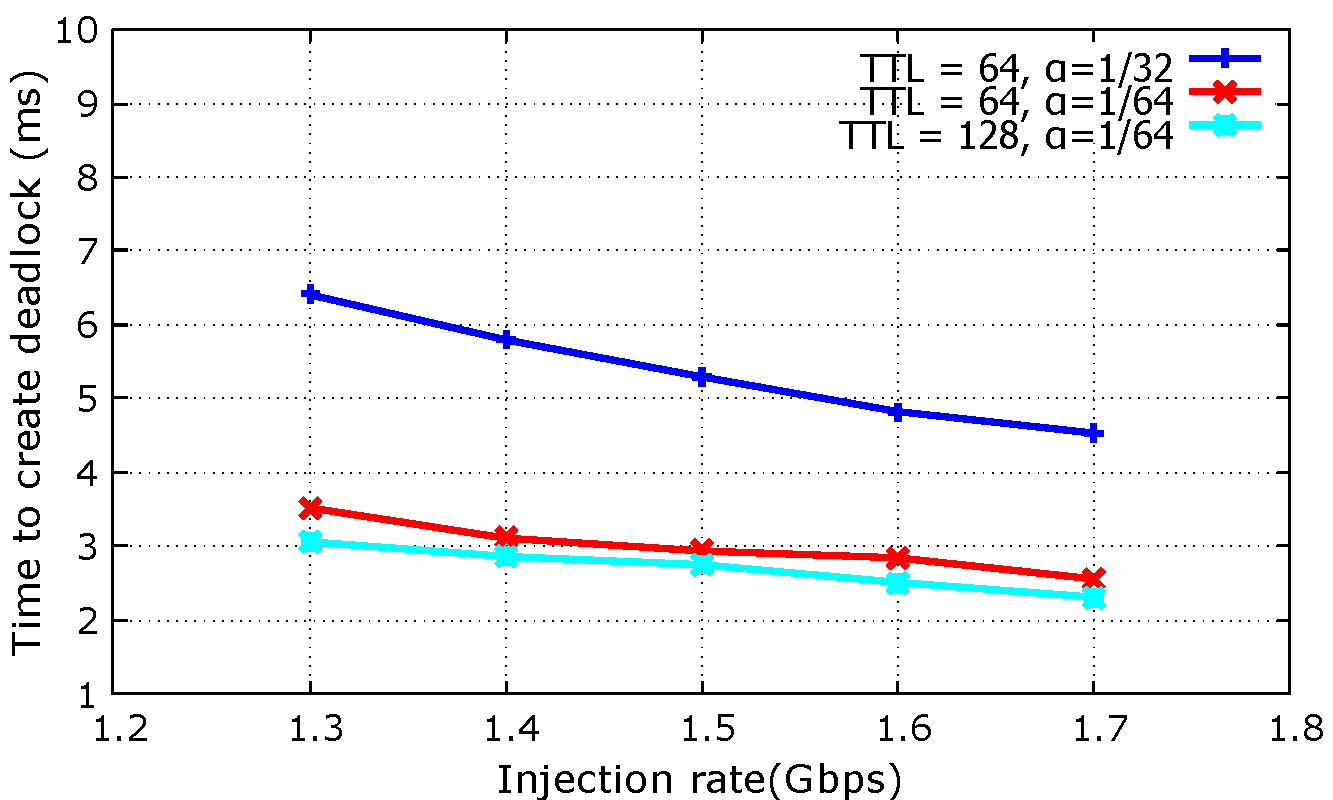
\includegraphics[width=0.5\textwidth,center]{figs/r_dltime.pdf}
%\caption[Optional caption for list of figures]{Measurement of the time to create a deadlock under different settings (deadlock will not occur when the injection rate is less than 1.3Gbps).}
%\label{fig:dltime_measurement}
%\end{figure}
%
%\parab{Measurement of the time to create a deadlock:} We manually configure a loop between two Arista 7050QX32 switches which have 32 full duplex 40Gbps ports and 12MB shared buffer. In Fig.~\ref{fig:dltime_measurement}, we set $\alpha$ and $TTL$ to different values and measure the time to create a deadlock under different injection rates.
%
%We can make four observations from the results in Fig.~\ref{fig:dltime_measurement}: 1) It takes only a few milliseconds to create a deadlock even when the injection rate is less than 2Gbps. This indicates that it is easy for a deadlock to occur even when only a transilient loop exists in the network. In addition, we cannot rely on any loop detection and recovery solutions to prevent the occurance of deadlocks as they are too slow to resolve the loop within a few milliseconds. 2) As the injection rate increases, the time to create a deadlock decreases accordingly. 3) Given a fixed injection rate, a smaller $\alpha$ value requires less time to create a deadlock. 4) Given a fixed injection rate, a smaller TTL value requires more time to create a deadlock. This is because a smaller TTL value will make the packets get dropped faster in the loop, and thus more packets are needed to be injected into the loop to trigger switch to pause each other.
%
%We repeated this experiment using many other combinations of TTL and $\alpha$ values and different number of switches. We found that all the results comply with what have been shown in Fig.~\ref{fig:dltime_measurement}.
%
%The takeaway of this experiment is that: once there is a loop in the network, deadlock is easy to occur and very hard to prevent (a deadlock can be created within a few milliseconds). In addition to a fast loop detection mechanism, we need an effective solution to detect and resolve deadlocks caused by all kinds of loops.

%\parab{Estimation of the time to create a deadlock:}

%\parab{Sufficient condition for deadlock creation:} \todo{(detailed content to be added later.)}
%
%   1. Analysis of the maximum packet drain rate caused by TTL expiration: $r^{max}_d = nB/k_ttl$.
%
%   2. Using testbed experiments to demonstrate that $r > r^{max}_d$ is a sufficient condition for deadlock creation.
%
%\parab{Creation time of deadlock:} \todo{(detailed content to be added later.)}
%
%   1. Analysis of the upper bound and lower-bound of the creation time of deadlock.
%
%   2. a) Using testbed experiments to demonstrate that lower-bound value is already a tight estimation when $r << B$; b) Analysis of the impact of PFC PAUSE frames on $r$ and $r^{max}_d$.
%
%\subsection{Analysis of device bug induced deadlock}\label{subsec:analysis_loop_deadlock}
%\todo{to be added.}

\secspace
\section{Potential Deadlock Mitigations}
\label{sec:mitigation}
\secspace

Since cyclic buffer dependency is a loose condition for deadlock, there are
mitigation mechanisms that avoid deadlock even if cyclic buffer dependency is present.
The examples and analysis in Section~\ref{sec:analysis}
inspire us with some of the following potential deadlock mitigations.


\para{TTL-based mitigation for deadlock caused by loops.} In a routing loop, 
the smaller TTL, the less possible deadlock forms (see Equation~\ref{eq:condition}).
Thus, the most straightforward mitigation is to reduce packets' initial TTL values.
For example, in an $N$-hop routing loop, if the initial TTL is not larger than $N$,
no deadlock will form because the deadlock threshold for $r$ is $B$, which can
never be exceeded.

In practice, we may not be able to guarantee that initial TTL values are always smaller than
the size of the loop. However, by proper switch buffer management, we may make {\em class-specific}
TTL much smaller than the actual TTL values. For example, if we assign packets 
that have different TTL values by at least $X$ to different priority classes, the effective TTL becomes $X$
within a priority class. Since PFC PAUSE operates based on priority classes, the deadlock threshold
of injecting rate $r$ is effectively increased.

In worst-case scenarios, the effective TTL may still be larger than the size of loop, meaning
that some $r$ smaller than $B$ leads to deadlock. We may consider rate limiting to keep
$r$ below the threshold $NB/TTL$, as discussed below.

\para{Rate limiting.} Commodity switches support bandwidth shaping for each priority class
or even particular flows. This can mitigate deadlock caused by both routing loops and multi-flow
buffer dependency, as shown in Section~\ref{sec:analysis}. If we are able to predict the rate 
threshold for deadlock, we may bound the individual flow rate by that threshold on switches 
that are involved in cyclic buffer dependency. However, this requires intelligent rate
limiting schemes to avoid over-punishing innocent flows. We leave this to future work.


\para{Limiting PFC pause frames near the source}
PFC is well known for its HoL blocking problem. The damage of HoL and the potential deadlock caused 
by PFC is significant because the pause frames are generated near the destination or in the middle of 
the network, where network congestions usually happen. Hence if we can limit the PFC pause frame 
generation near the source, we can reduce the damage of both deadlock and HoL blocking. 

Here we describe several possible ways of doing so: first, we can assign different PFC thresholds to 
the ports of a switch based on their positions. Ports connecting to the downstream get smaller threshold, 
whereas ports connecting to the upstream get larger threshold. 
Second, we can use switches with larger threshold values at the higher tiers so that they can absorb 
temporal burstiness instead of generating PFC pause frames. Third, again, we may classify 
packets with different TTL into different classes and assign them different PFC thresholds.
Unfortunately, these solutions may lead to other issues including the unfairness between long (across 
different high tier switches) and short ({\em e.g.,} within the same rack) flows. 
This trade-off is less understood and worthy of further study.

% using larger threshold values is tricky, 
%as it does not push PFC back to the source for all cases.)

%In Clos networks, a deadlock that involves high tiers can cause the most serious damage.
%A natural mitigation is to limit the impact of PFC locally near servers. This reduces
%the risk of deadlock as well as the impact once deadlock occurs.
%The idea is to assign different PFC thresholds to different tiers and make PFC happen less
%on higher tier. Also, higher tier switches may be allowed to ignore PFC or drop packets from
%lower tier upon extreme cases.
%The price is that this turns the network into partly
%``lossy'' and may cause congestion drops.

%Second, we may classify packets based on the TTL value they carry, and use TTL-based buffer 
%management similar to that in \ref{karol2003prevention}. The smaller the TTL value of a packet, 
%the smaller the chance that the packet will trigger PFC pause frames. Hence the TTL-based buffer 
%management has the ability to limiting the pause frame generation near the source. But its fairness 
%property is less understood and worthy of further study.

\para{Preventing PFC from been generated.}
The recent transport protocols, DCQCN~\cite{dcqcn} and TIMELY~\cite{timely} are designed to reduce 
the possibility of PFC generation. But due to the feedback 
latency introduced by the end-to-end delay, and the fact that both algorithms react only after the 
congestions have been generated (through either queue length or latency increase), they cannot prevent PFC 
from been generated. 

One possible way to further preventing PFC from been generated is to integrate DCQCN together with 
phantom queuing, like~\cite{Alizadeh12}. By reacting to the phantom queues that assume lower link speed, 
congestion signals are generated much earlier. 

\para{Other possible mechanisms.} In future work, a deeper understanding of tighter conditions 
for deadlock may lead to more deadlock mitigation mechanisms. In future work, we are going to 
investigate the tightest possible conditions -- necessary and sufficient condition for deadlock. 
%\vspace{-0.1in}
\section{Related Work}\label{sec:related}

\para{Deadlock-free routing.} Many Deadlock-free routing designs have been
proposed. See
\cite{dally,duato93,dally93,sancho2004,flich2012survey,lash,wu2003fault,glass,duato2001,domke2011,puente1999,dfedst16}
for representative schemes. Generally, these designs prevent deadlock by
imposing restrictions on the routing paths, and can be classified into two
categories.

The first category is {\em deterministic routing based approach}, in which the
routing path is not affected by the traffic status, and there is no CBD.  These
routing algorithms are not compatible with existing routing protocols including
OSFP and BGP. Worse, they cannot be implemented in current commodity switching
ASICs.

TCP-Bolt~\cite{tcpbolt} and DF-EDST~\cite{dfedst16} are two recently
proposed deadlock-free routing designs. They both build edge-disjoint
spanning trees (EDSTs), with DF-EDST~\cite{dfedst16} further builds a
deadlock-free tree transition acyclic graph such that the transition
among some EDSTs can be allowed. However, existing L3 routing protocols
do not guarantee that packets will follow the pre-assign EDSTs, especially
upon link failures. Current switching ASIC cannot detect and handle all 
the potential EDST transition properly.

%support EDST.
%Furthermore, these designs need many EDSTs and
%every EDST needs to occupy a lossless queue. 
%Current switching ASIC,
%however, can only support 2-3 lossless queues.

The second category is {\em adaptive routing based approach.} The key idea is to
pre-install  ``escape'' paths at every switch to cover all possible
destinations. The switches can reroute packets to the ``escape'' paths in the
presence of congestion so that deadlock can be avoided.  As far as we know, no
commodity switching ASIC supports dynamic reroute based on traffic / queue
status.

\para{Intel Omni-Path.} Intel Omni-Path architecture \cite{omnipath} uses the
concept of Service Channels (SC) for routing deadlock avoidance.  Unlike
\sysname{}, Ommi-path uses a centralized fabric manager to manage the
network~\cite{omnipath}, including setting up SCs. This is not feasible at
data center scale.

%% Technical details of Omni-Path are not currently available, Tagger differs
%% from Omni-Path in two significant ways. First, Omni-path needs a fabric
%% manager to dynamically setup SC whereas the tag match-action rules are
%% pre-computed and statically configured. Second, Tagger enforces that
%% the tag of a packet increases monotonically whereas Omni-Path does not
%% enforce order for SC.

\para{Buffer management for deadlock prevention.} It has been shown that by
increasing the packet priority hop-by-hop, and putting packets of different
priority into different buffers, deadlock can be avoided
\cite{firstpaper,survey,datanetworks,karol2003prevention}. These designs,
however, need a large number lossless queues (which is the diameter of the
network). In \cite{dag}, the author tried to reduce the number of lossless
queues to only two. The design does not guarantee losslessness. Furthermore,
some switches need much larger buffer space than the others. 

\para{Deadlock recovery.} Deadlock recovery schemes
\cite{isca95,shpiner2016unlocking,venkatramani1996,martinez1997,Lopez1998}
detect deadlocks once they occur, and then try to break them by rerouting
packets.  These approaches have two issues: (1) They cannot guarantee that
deadlock will not happen again (if they can, there will be no need for deadlock
recovery). (2) They cannot be deployed using existing switch hardware.

%% need to add new deadlock detection algorithms and deadlock
%% breaking protocols into the switches.

%\para{Circuit switching-based approaches.} Those solutions from HPC and InfiniBand
%work by preemption. This does not work in Ethernet and in practice.

\para{Deadlock-free routing reconfiguration}:
Several deadlock-free routing reconfiguration schemes
\cite{automatic,lysne2005,doublescheme,gara2005} have been proposed for
ensuring deadlock-free during routing reconfiguration. \sysname{} can
be used to help any routing protocol to be deadlock-free, as
\sysname{} is decoupled from the routing protocols.

%The basic idea is to divide the reconfiguration process into multiple
%stages, and guarantee deadlock-free routing within each stage. We
%believe
%\sysname{} can be easily modified to guarantee deadlock-free of each
%reconfiguration stage.

\para{Summary.} \sysname{} is different from prior work because it works with
any routing protocol, and with existing hardware. We further have shown that
\sysname{} needs only small number of lossless queues.

%We believe that deciding the priority of packets along the path is
%better than changing routing configurations.

%Deadlock-free routing \cite{dally,duato93,dally93,sancho2004,flich2012survey,lash,wu2003fault,glass,duato2001,domke2011,puente1999} can be achieved by splitting the physical links into virtual channels and virtual channels are arranged in a way so as to avoid circular buffer dependency. In all those designs, the routing is decided by the virtual channels. Hence they cannot work with existing routing protocols for the data center networks which was designed for the lossy networks.
%can be achieved by splitting the physical links into virtual channels and virtual channels are arranged in a way so as to avoid circular buffer dependency. In all those designs, the routing is decided by the virtual channels. Hence they cannot work with existing routing protocols for the data center networks which was designed for the lossy networks.

%%TCP-Bolt~\cite{tcpbolt} uses multiple edge-disjoint spanning trees (EDSTs) and puts every EDST into a separate VLAN and lossless queue to achieve deadlock-free. In addition to the above drawbacks, to achieve good performance, TCP-Bolt may need a large number of lossless queues (which cannot be provided in current commodity switches). Furthermore, TCP-Bolt needs to run layer-2 VLAN, whereas all large-scale data center networks run layer-3.
%
%%DF-EDST~\cite{dfedst16} introduces a set of edge-disjoint spanning trees and a tree transition graph to provide deadlock free routing for arbitrary data center network topologies. DF-EDST, however, cannot work with existing routing protocols as it needs to follow the EDSTs. Furthermore, The EDST selection and transition cannot be readily implemented in current Ethernet switches.

\secspacelarge
\section{Conclusion}
\secspace

In this paper, we studied the problem of deadlock in datacenter networks.  We
showed that CBD is a {\em necessary} by not {\em
sufficient} condition for deadlock formation. We are unable to fully characterize
the sufficient conditions, but using insights gained from a few examples, we
discussed potential deadlock mitigation mechanisms including TTL-based schemes,
rate limiting and reducing PFC propagation.


%\vspace{0.1in}
%\section*{Acknowledgements}


%\begin{normalsize}
%\begin{small}
\bibliographystyle{plain}
\bibliography{reference}
%\end{small}
%\end{normalsize}
%\begin{appendices}
\section{PFC headroom calculation}\label{APPHEADROOM}

The PFC headroom needed per port per lossless queue can be calculated by
		considering the time interval needed for a receiver to pause its
		upstream sender. The time interval is composed of the following 6
		periods for the lossless class $p$:

	
\noindent\textbf{The time to send a PAUSE frame $t_1$}.  Once a pause frame is
		generated, it may be blocked by a packet that has just started
		transmision. Since Ethernet is non-preemptive, in the worst-cast,
		$t_1 = \frac{ L_{mtu} + L_{pfc}}{B}$, where $L_{mtu}$ is the MTU size,
		and $L_{pfc}$ is the size of a PFC pause frame, and $B$ is the link
		rate.


\noindent\textbf{The PAUSE frame propagation time $t_2$}. This depends on 
		the cable length between the sender and receiver.

\noindent\textbf{The PAUSE frame receiving time at the sender $t3$}.
		$t_3=\frac{L_{pfc}}{B}$.

\noindent\textbf{The PFC response time $t_4$}. This is the amount of time needed
		for the sender to process the pause frame.

\noindent\textbf{The time for the sender to stop transmitting $t_5$}. Again,
		because Ethernet is non-preemptive, sender must to finish 
		transmitting the packet that may have already started. Hence, in the
		worst case, $t_5 =
		\frac{L^{p}_{mtu}}{B}$.

\noindent\textbf{The time for the pipe to be drained $t_6$}. We know $t_6 =
		t_2$.


At a first glance, the headroom size should be $B\times\sum t_i$. But there are
some additional details. The switching ASICs typically divide a packet
into small cells of equal size for internal packet storage and
processing. The cell size ($C$) is typically larger than the smallest
Ethernet packet size (64 bytes). For one 64-byte packet, one cell is
allocated. So in the worst-case, the needed headroom size is:
\begin{eqnarray} \label{eqn:pfcheadroom} S_{hdr} & = &
C\lceil\frac{(t_1+t_2+t_3+t_4 + t_6)B}{64}\rceil + C\lceil \frac{t_5
B}{64}\rceil \nonumber \end{eqnarray}

For a typical 40GbE RoCEv2 setup, we have $L_{mtu}=1500$ bytes, $L_{pfc}=64$
bytes, $t_2=t_6=1us$ (for about 200 meters cable length), $t_4=2.75us$,
$L^{p}_{mtu}=1100$ bytes, $C=208$ bytes.  For a commodity switch with 32
full duplex 40GbE ports, the total headroom size needed is 2.76MB for
supporting one lossless queue.  

\section{Optimal tagging scheme for Clos network}
\label{sec:clos_optimal}

Algorithm~\ref{alg:clos} produces optimal tagging for Clos networks. Note
similarity to Algorithm~\ref{alg:ttl}, except for the last step, which is
specific to Clos networks.

\begin{algorithm}
	\small
    \KwIn{Clos topology and lossless routes $R$}
	\KwOut{A tagged graph $G(V, E)$}
	$V \gets Set()$\;
	$E \gets Set()$\; 
	\For{each path $r$ in $R$} {
		$tag \gets 0$\;
		\For{each hop $h$ in $r$} {
			$V \gets V \cup \{(h, tag)\}$\;
			$E \gets E \cup \{lastHop\rightarrow(h, tag)\}$\;
			\If{$h$ is going down \&\& nextHop is going up} {
				$tag \gets tag+1$\;
			}
		}
	}
	\Return{$G(V, E)$}\;
    \caption{The optimal tagging system for Clos topology.}
	\label{alg:clos}
\end{algorithm}
\end{appendices}


\end{document}
